\documentclass[letterpaper, 11pt]{article}
\usepackage{comment} % enables the use of multi-line comments (\ifx \fi) 
\usepackage{fullpage} % changes the margin
\usepackage{fancyhdr} % for footer
\usepackage[UKenglish]{isodate}% http://ctan.org/pkg/isodate for date format
%\usepackage{fixltx2e}%subscript
\usepackage{float}%force tables/figs into certain placement
\usepackage{changepage}%for dichotomous key
\usepackage{graphicx}%for figures
\usepackage{subcaption}%for figures
\usepackage{hyperref}%for links
\usepackage[font=small,labelfont=bf]{caption}%for captions
\usepackage[letterpaper,margin=1in]{geometry}
\usepackage{placeins}%prevent images from floating into inappropriate sections
\usepackage{multicol}				% 2-column layout
\usepackage{natbib}	%for bibliography

\def\labelitemi{--}

\pagestyle{fancy}
\renewcommand{\headrulewidth}{0pt}
%
\lhead{}
\chead{}
\rhead{}
\lfoot{ENT 432 (Fall 2016) - Penn State}
\cfoot{}
\rfoot{\thepage}
\renewcommand{\footrulewidth}{0.4pt}
\title{Unit 15 - Amphiesmenoptera}
\author{Andrew R. Deans and Istv\'an Mik\'o}

\begin{document}
\cleanlookdateon %removed ordinal date
\maketitle
\thispagestyle{fancy}

\section*{Introduction}
\textbf{Amphiesmenoptera} comprises two familiar orders, Lepidoptera (moths and butterflies; covered in section 1) and Trichoptera (caddisflies; section 2), whose close relationship is uncontroversial. To open this unit we'll discuss the evolutionary significance of two characteristics shared by these insects: silk production (from the labium) and possession of setiferous wings.

%All families we cover in lab are classified in the suborder \textbf{Glossata}, the lepidopterans that possess, at least ancestrally (lost in some groups), a coilable proboscis.

\section*{Materials}
\begin{itemize}
\item specimens (provided)
\item fine forceps, probes (provided)
\item sorting tray, watch glasses, gloves, safety glasses, glycerine, ethanol (provided)
\item pencil/paper for sketches
\end{itemize}

\section*{Safety}
We will be working with sharp tools and insects on pins. Wear your personal protective gear at all times. Specimens are to be returned to their vials after lab, and glycerine and ethanol will be collected for proper disposal or reuse.

\section*{Methods}
Working with a partner, organize your space, specimens, tools, and microscope. Use your probe and forceps to manipulate the specimen. In this lab, however, we will not be dissecting specimens (unless otherwise noted). Wing venation is especially useful, and one can see these characters more clearly by placing one or two drops of ethanol on the wing. The wing color and pattern should remain unchanged after the ethanol evaporates. You can start anywhere in the handout.

\section{Lepidoptera}

\noindent{}\textbf{Lepidoptera} is one of the ``big four'' orders of insects, and with \textgreater157,000 described species and at least 350,000, probably many more, remaining to be described. These insects are commonly referred to as moths and butterflies, and they remain one of the most recognizable groups of insects. Family-level diagnostics can be difficult, however, given that many characters are obscured by scales. The vast majority of species feed on plants as larvae (caterpillars), and adults live on liquid diets, imbibed through coiled, siphon-like mouthparts (proboscis, formed from the galeae). In adults, the hind wings of most species (\textit{i.e.}, the taxon Heteroneura) are of a different shape (usually shorter and more rounded) and venation than the fore wings.

\subsection*{Big picture questions}
\noindent{}What factors contribute to the overall diversity of Lepidoptera? Can you describe one or two characteristics that could be key innovations or opportunities? \\

\noindent{}Dytrisian taxa exhibit enormous diversity of larval integumentary modifications. Why are larvae of non-dytrisian generally less distinct? \\

\noindent{}Can you provide  two examples of antipredator adaptations, related to the modified wing setae? \\

\noindent{}What are the precursors of tympana? Do you think the ``ears'' on different body regions in different lepidopterans are homologous? \\ 

\noindent{}What trends do we see across the phylogeny of Lepidoptera, with respect to feeding biology, mouthpart morphology, and wing morphology? \\

\noindent{}Familiarize yourself with the following taxon names, which refer to organisms you are likely to encounter in the northeastern USA and/or which are phylogenetically relevant. Can you describe how these arthropods live (natural history) and roughly how diverse they are? Do you know how they're related to one another? If you had to choose a family to study from the taxa below which one would it be and why?

\begin{enumerate} 
\item Amphiesmenoptera
\item Ditrysia
\item Rhopalocera
\item Micropterigidae
\end{enumerate}

\subsection{Non-dytrisian Lepidoptera (``Monotrysia'')}
There is one family of commonly encountered moths that each have a single opening at the apex of its abdomen, for copulation and oviposition.

\subsubsection{Nepticulidae (serpentine leafminer moths)}
\noindent{}\textit{Diagnostic characters:} Wingspan 3.5--10 mm, among the very smallest of moths; usually black and white, with a metallic band or gold speckles; antennae with an eye cap; maxillary palps well developed, long and folded; fore wing with branched veins.\\

\noindent{}\textit{Natural history:} Larvae make thin, winding mines on the leaves of trees and shrubs. There are roughly 800 described species.

\begin{figure}[ht!]
    \centering
    \begin{subfigure}[ht!]{0.4\textwidth}
        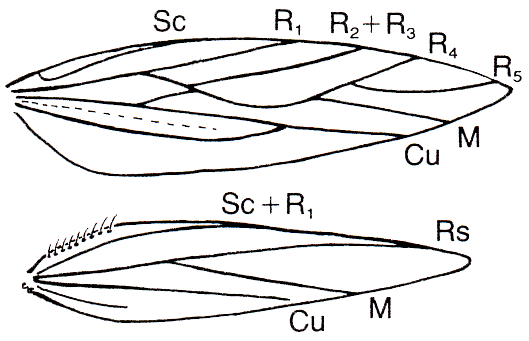
\includegraphics[width=\textwidth]{image29}
        \caption{Wings}%need new image; this is copyright
        \label{fig:nepticulid2}
    \end{subfigure}
    \qquad %add desired spacing between images, e. g. ~, \quad, \qquad, \hfill etc. 
      %(or a blank line to force the subfigure onto a new line)
    \begin{subfigure}[ht!]{0.45\textwidth}
        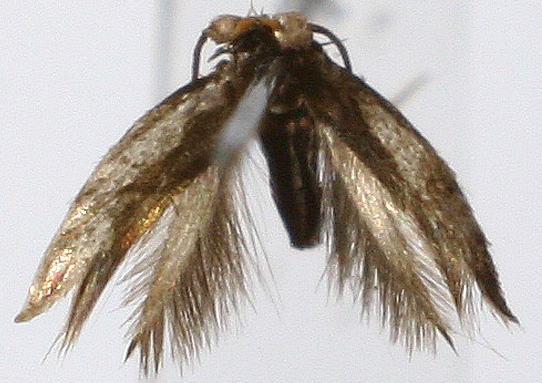
\includegraphics[width=\textwidth]{nepticulid1}
        \caption{Habitus. Photo CC0 by M. Virtala \url{https://goo.gl/esgiwJ}}
        \label{fig:nepticulid1}
    \end{subfigure}
    \caption{Nepticulidae}\label{fig:nepticulids}
\end{figure}

\subsection{Dytrisia}
The remaining lepidopterans, \textgreater98\% of all species, are classified in an unranked (sometimes a ``division''), monophyletic taxon called Ditrysia. These insects have separate openings for copulation and oviposition.

\subsubsection{Gracillariidae (blotch leafminer moths)}
\noindent{}\textit{Diagnostic characters:} Minute to small in size (wingspan 5--20 mm); often brightly colored or metallic; maxillary palps usually absent;  proboscis bare; wing venation reduced and elongate proximally, wing fringe long; hind wing lanceolate.\\

\noindent{}\textit{Natural history:} 

\begin{figure}[ht!]
    \centering
    \begin{subfigure}[ht!]{0.4\textwidth}
        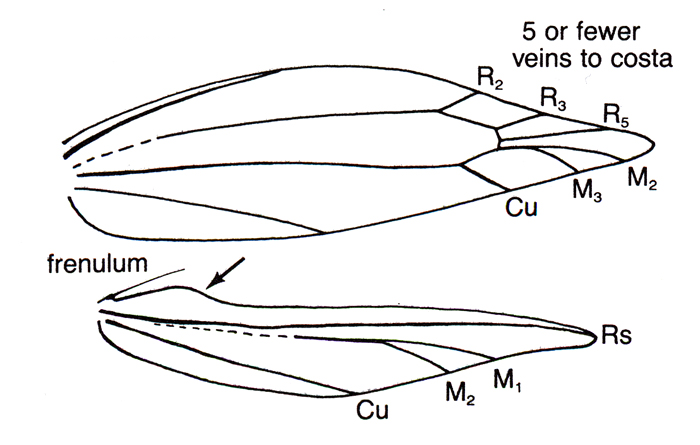
\includegraphics[width=\textwidth]{image33}
        \caption{Wings}%copyrighted image
        \label{fig:gracill1}
    \end{subfigure}
    \qquad %add desired spacing between images, e. g. ~, \quad, \qquad, \hfill etc. 
      %(or a blank line to force the subfigure onto a new line)
    \begin{subfigure}[ht!]{0.45\textwidth}
        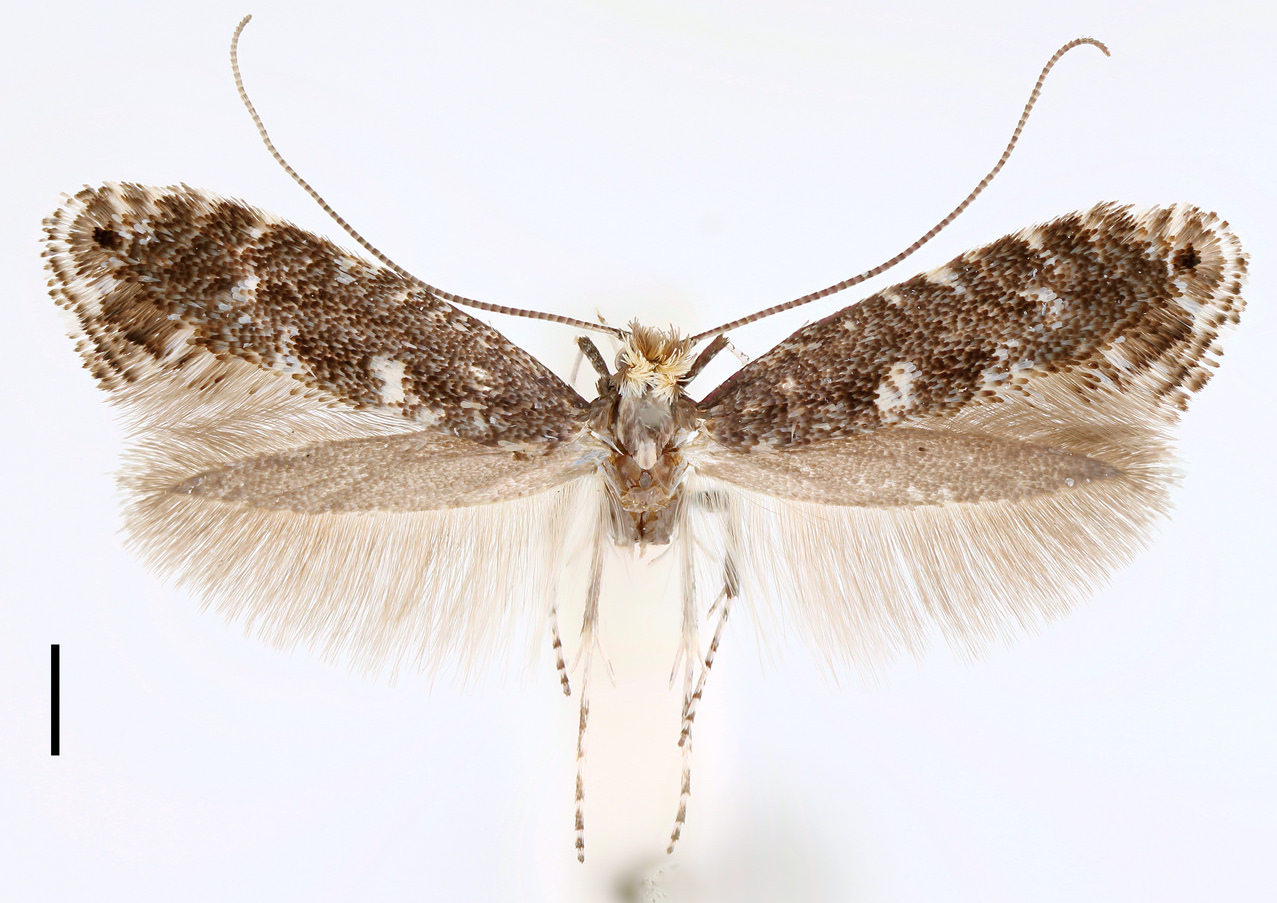
\includegraphics[width=\textwidth]{gracil}
        \caption{Habitus. Photo (CC BY-NC 2.0) by Museum of Zoology, Lund University: Entomology \url{https://flic.kr/p/pfEv2z}}
        \label{fig:gracill2}
    \end{subfigure}
    \caption{Gracillariidae}\label{fig:gracillariids}
\end{figure}

\subsubsection{Gelechiidae (twirler moths, leaf tiers)}
\noindent{}\textit{Diagnostic characters:} Small (wingspan 7--25 mm); maxillary palps short, 4-segmented, located close to base of proboscis; labial palps long, upcurved, 3rd segment elongate and tapering; proboscis scaly; hind wing drawn out to a point anteriorly at apex, so that tip of wing is concave.\\

\noindent{}\textit{Natural history:} 

\begin{figure}[ht!]
    \centering
    \begin{subfigure}[ht!]{0.45\textwidth}
        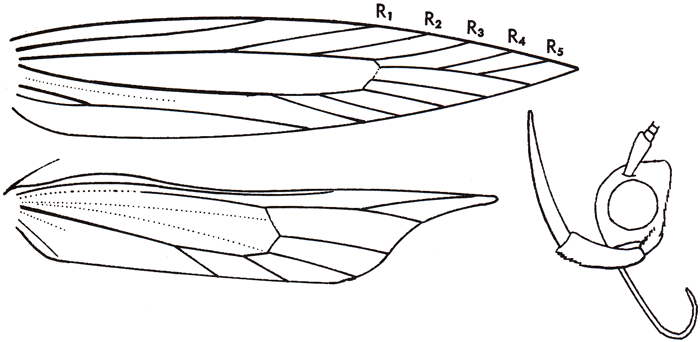
\includegraphics[width=\textwidth]{image35}
        \caption{Wings (left), head with palp (right)}
        \label{fig:gelechiid1}
    \end{subfigure}
    \qquad %add desired spacing between images, e. g. ~, \quad, \qquad, \hfill etc. 
      %(or a blank line to force the subfigure onto a new line)
    \begin{subfigure}[ht!]{0.45\textwidth}
        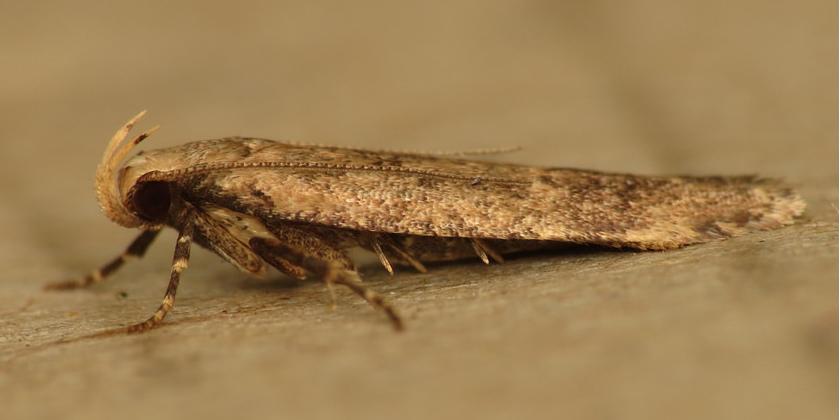
\includegraphics[width=\textwidth]{gelechiid}
        \caption{Habitus. Photo (CC BY 2.0) by Donald Hobern \url{https://flic.kr/p/o4Um8Z}}
        \label{fig:gelechiid2}
    \end{subfigure}
    \caption{Gelechiidae}\label{fig:gelechiids}
\end{figure}

\subsubsection{Tineidae (clothes moths and relatives)}
\noindent{}\textit{Diagnostic characters:} Small to medium-sized (wingspan 7--36 mm), usually gray or brown; head vestiture entirely comprised of erect scales (bushy); antennae with a whorl of erect scales on each segment; maxillary palps usually present, folded; labial palps with sparse, elongate spines, usually very obvious; wing venation not so reduced as in above families.\\

\noindent{}\textit{Natural history:} 

\begin{figure}[ht!]
    \centering
    \begin{subfigure}[ht!]{0.45\textwidth}
        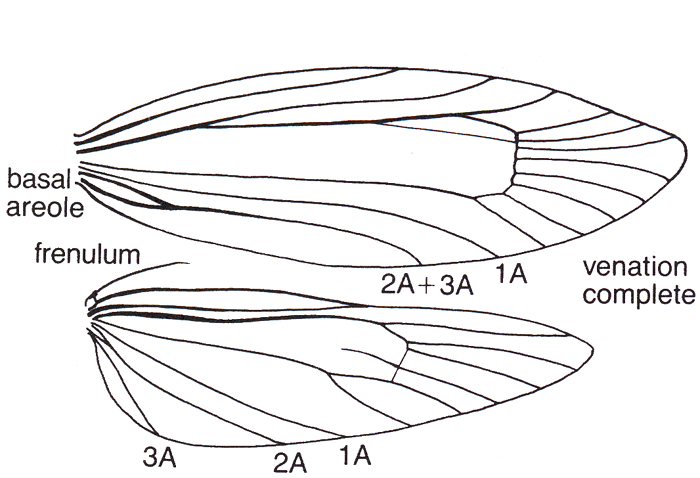
\includegraphics[width=\textwidth]{image34}
        \caption{Wings}
        \label{fig:tineid1}
    \end{subfigure}
    \qquad %add desired spacing between images, e. g. ~, \quad, \qquad, \hfill etc. 
      %(or a blank line to force the subfigure onto a new line)
    \begin{subfigure}[ht!]{0.45\textwidth}
        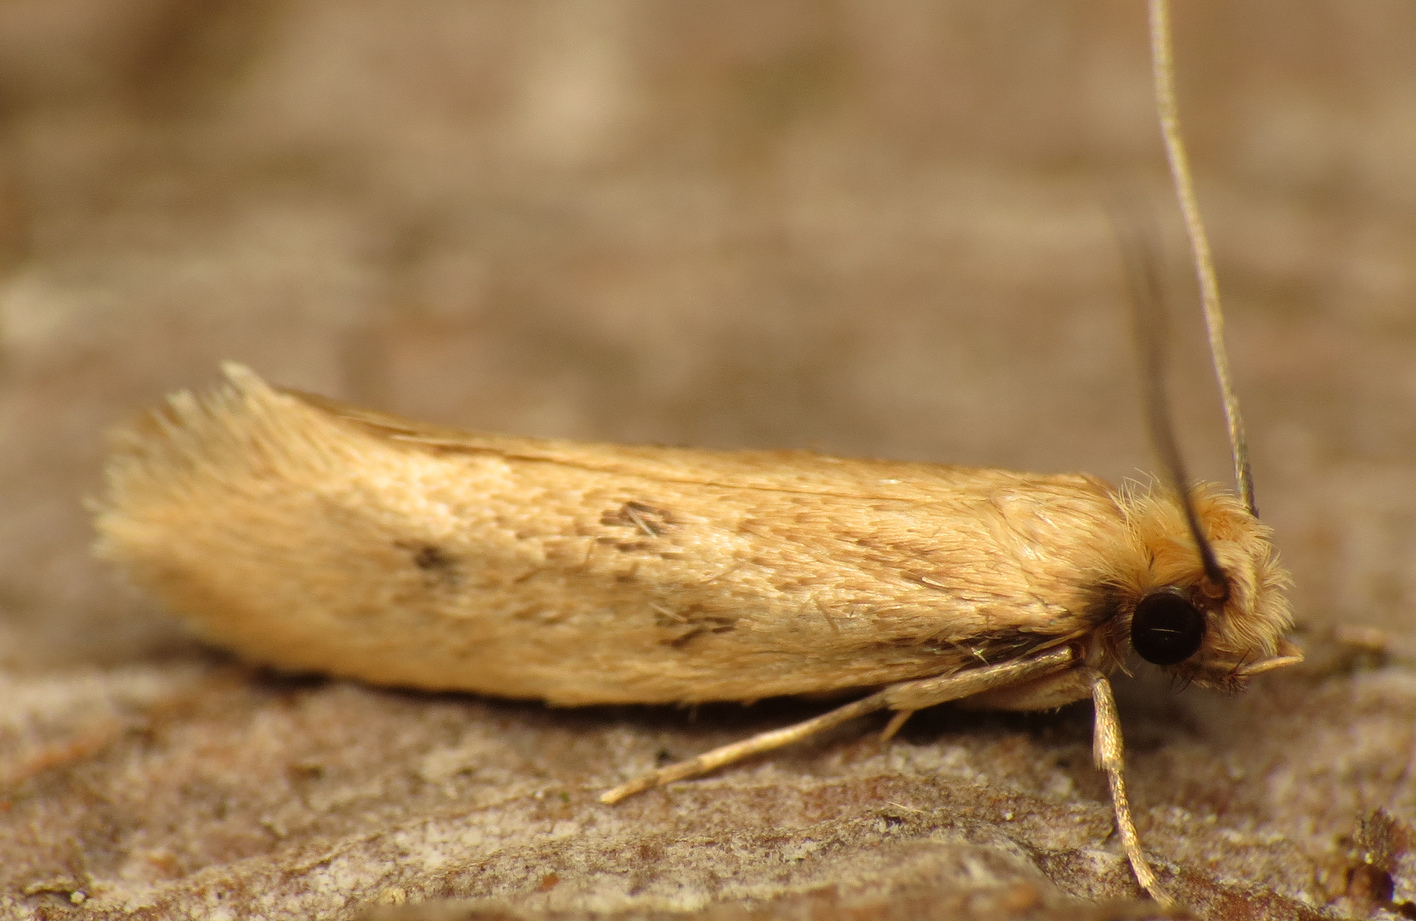
\includegraphics[width=\textwidth]{tineid1}
        \caption{Habitus. Photo (CC BY 2.0) by Donald Hobern \url{https://flic.kr/p/eiZu6Y}}
        \label{fig:tineid2}
    \end{subfigure}
    \caption{Tineidae}\label{fig:tineids}
\end{figure}

\noindent{}Note that the remaining families usually have more obvious morphological differences between the fore wing and hind wing, mainly that the hind wing is wider when measured along the anterior-posterior axis.

\subsubsection{Attevidae}
\noindent{}\textit{Diagnostic characters:} Small to medium-sized (wingspan 8--31 mm), slightly narrow-winged moths; often brightly colored; wing tips relatively blunt; head and labial palps with smooth scales; ocelli absent; maxillary palps have 1--2 segments

\noindent{}\textit{Natural history:} 

% Might be good to add Pterophoridae too - easy to ID and fairly common. - Chris Grinter

\begin{figure}[ht!]
    \centering
    \begin{subfigure}[ht!]{0.36\textwidth}
        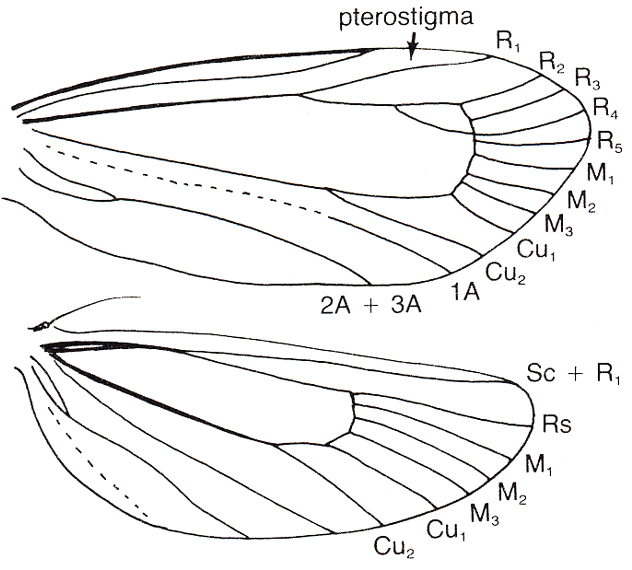
\includegraphics[width=\textwidth]{image40}
        \caption{Wings}
        \label{fig:attev1}
    \end{subfigure}
    \qquad %add desired spacing between images, e. g. ~, \quad, \qquad, \hfill etc. 
      %(or a blank line to force the subfigure onto a new line)
    \begin{subfigure}[ht!]{0.45\textwidth}
        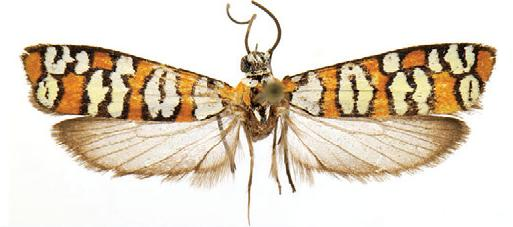
\includegraphics[width=\textwidth]{ypono}
        \caption{Habitus. \citep[Photo CC BY 3.0 by ][]{wilsonetal2010}}
        \label{fig:attev2}
    \end{subfigure}
    \caption{Attevidae}\label{fig:attevids}
\end{figure}

\subsubsection{Psychidae (bagworm moths)}
\noindent{}\textit{Diagnostic characters:} Small to medium-sized moths (wingspan 12--36 mm); body usual black in North American species; wings often absent or reduced in females, which remain in the silken bag (Figure \ref{fig:psychid2}); male wings often (but not always!) mostly clear; setae hair-like, rather than scale-like.\\

\noindent{}\textit{Natural history:} Larvae form bags constructed of silk and plant material.

\begin{figure}[ht!]
    \centering
    \begin{subfigure}[ht!]{0.36\textwidth}
        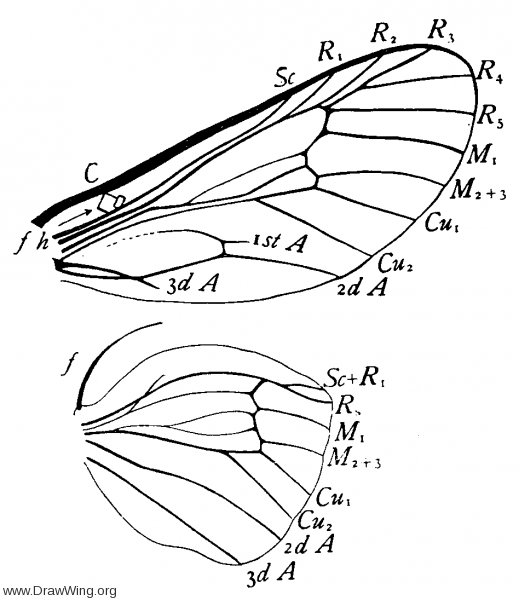
\includegraphics[width=\textwidth]{PsychidWings}%fig 46 from Comstock 1918
        \caption{Wings}
        \label{fig:psychid1}
    \end{subfigure}
    ~ %add desired spacing between images, e. g. ~, \quad, \qquad, \hfill etc. 
      %(or a blank line to force the subfigure onto a new line)
    \begin{subfigure}[ht!]{0.15\textwidth}
        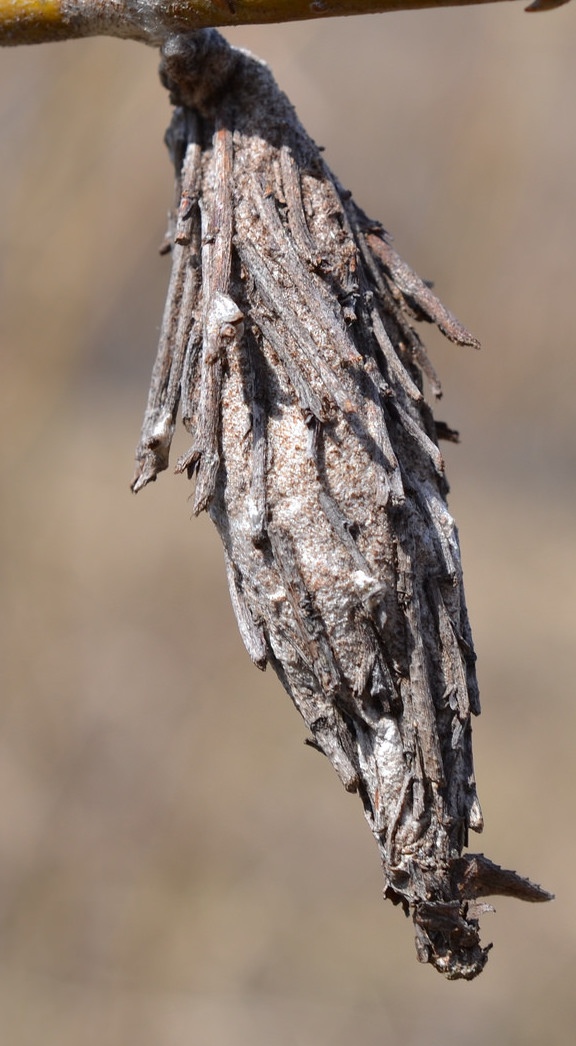
\includegraphics[width=\textwidth]{psychid2}
        \caption{Silken bag. Photo (CC BY 2.0) by Andrew C \url{https://flic.kr/p/mhAUfF}}
        \label{fig:psychid2}
    \end{subfigure}
    ~ %add desired spacing between images, e. g. ~, \quad, \qquad, \hfill etc. 
      %(or a blank line to force the subfigure onto a new line)
    \begin{subfigure}[ht!]{0.35\textwidth}
        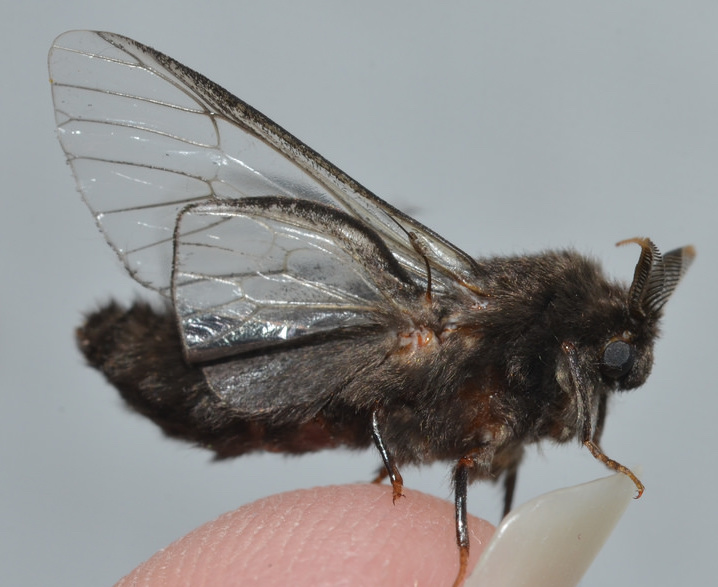
\includegraphics[width=\textwidth]{psychid1}
        \caption{Habitus. Photo (CC BY 2.0) by Andy Reago \& Chrissy McClarren \url{https://flic.kr/p/wZ8xCg}}
        \label{fig:psychid3}
    \end{subfigure}
    \caption{Psychidae}\label{fig:psychids}
\end{figure}

\subsubsection{Sesiidae (clearwing moths)}
\noindent{}\textit{Diagnostic characters:} Small to medium-sized (wingspan 15--50 mm); transparent, scaleless ``windows'' usually present on wings; often wasp-like in shape and color; antennae widen apically, but narrow at the apex and are often somewhat hooked.\\

\noindent{}\textit{Natural history:} 

\begin{figure}[ht!]
    \centering
    \begin{subfigure}[ht!]{0.45\textwidth}
        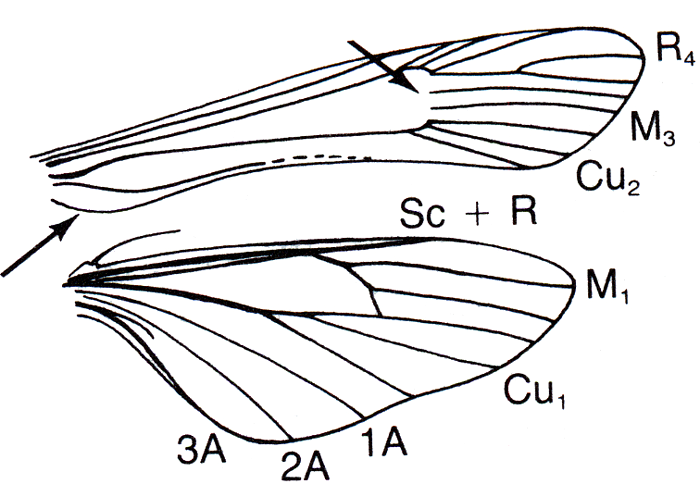
\includegraphics[width=\textwidth]{image42}
        \caption{Wings}
        \label{fig:sesiid1}
    \end{subfigure}
    \qquad %add desired spacing between images, e. g. ~, \quad, \qquad, \hfill etc. 
      %(or a blank line to force the subfigure onto a new line)
    \begin{subfigure}[ht!]{0.45\textwidth}
        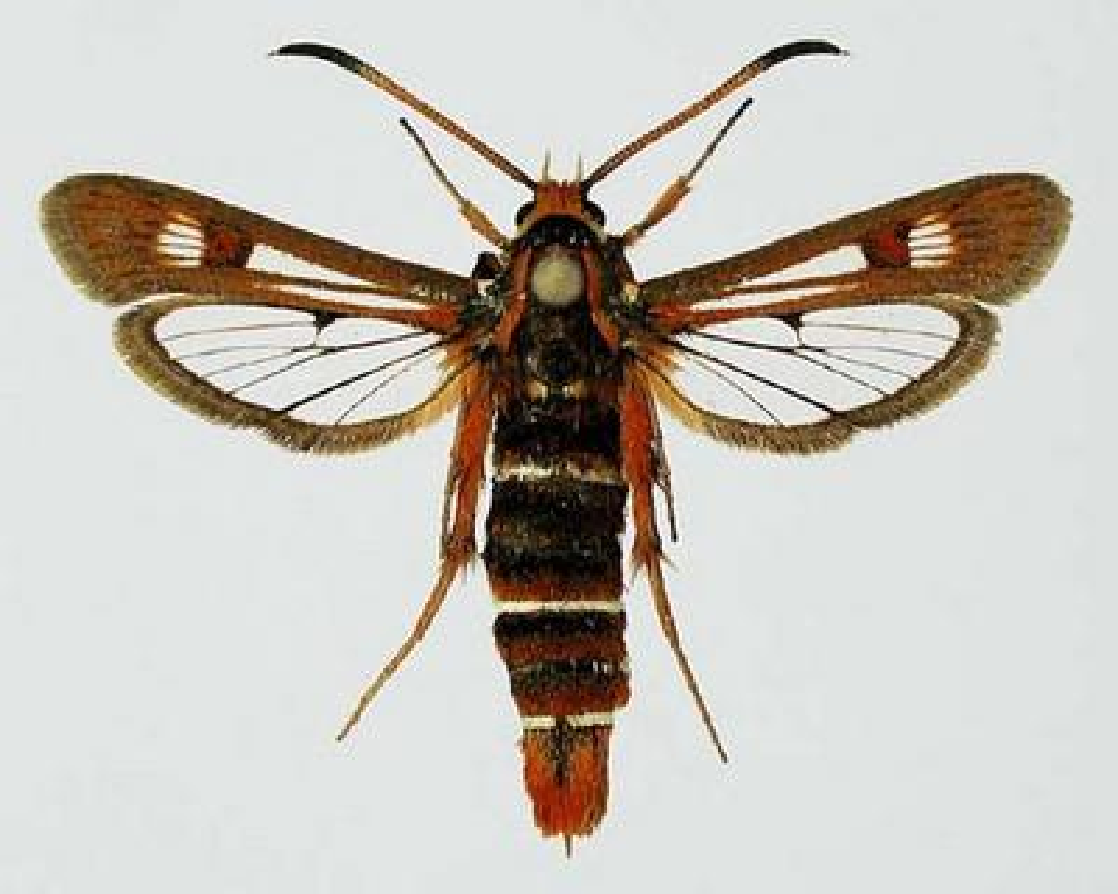
\includegraphics[width=\textwidth]{image41}
        \caption{Habitus}
        \label{fig:sesiid2}
    \end{subfigure}
    \caption{Sesiidae}\label{fig:sesiids}
\end{figure}

\subsubsection{Cossidae (carpenterworm moths)}
\noindent{}\textit{Diagnostic characters:} Relatively large (wingspan 30--100 mm), heavy-bodied; male antennae bipectinate, females filliform; species in the U.S. usually black and gray, dull or with some orange; head is relatively small compared to the rest of the body (as opposed to Sphingidae).\\

\noindent{}\textit{Natural history:} 

\begin{figure}[ht!]
    \centering
    \begin{subfigure}[ht!]{0.38\textwidth}
        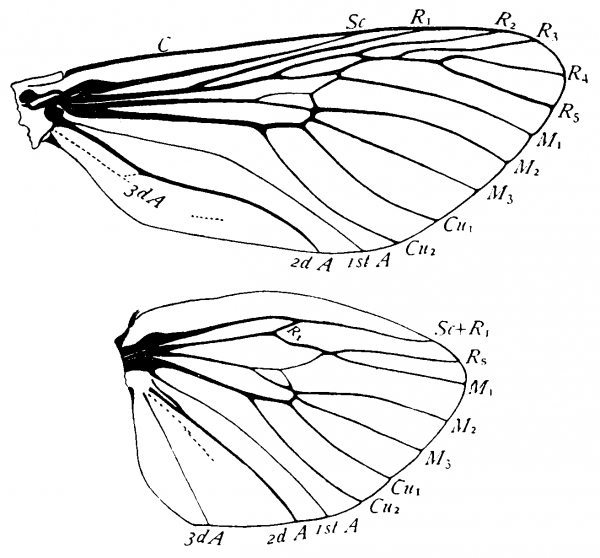
\includegraphics[width=\textwidth]{CossidWings}
        \caption{Wings \citep[Fig. 343]{comstock1918wings}}
        \label{fig:cossid1}
    \end{subfigure}
    \qquad %add desired spacing between images, e. g. ~, \quad, \qquad, \hfill etc. 
      %(or a blank line to force the subfigure onto a new line)
    \begin{subfigure}[ht!]{0.48\textwidth}
        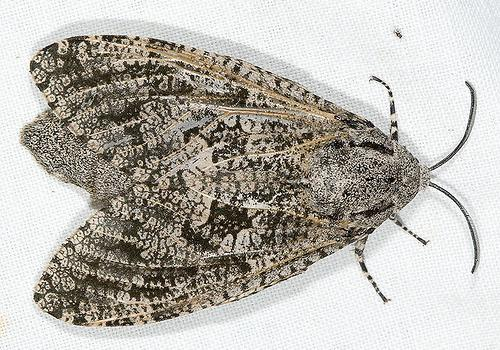
\includegraphics[width=\textwidth]{image43}
        \caption{Habitus}
        \label{fig:cossid2}
    \end{subfigure}
    \caption{Cossidae}\label{fig:cossids}
\end{figure}

\subsubsection{Tortricidae (leafroller and fruitworm moths)}
\begin{itemize}
\item fore wings broad, somewhat ``round-shouldered'', with squared-off tips
\item labial palps usually project forward, maxillary palps small
\item portions of scales on head often flattened
\item small to medium-sized (10--33 mm)
\item often with complex patterns on fore wings and plain hind wings
\end{itemize}

\begin{figure}[ht!]
    \centering
    \begin{subfigure}[ht!]{0.35\textwidth}
        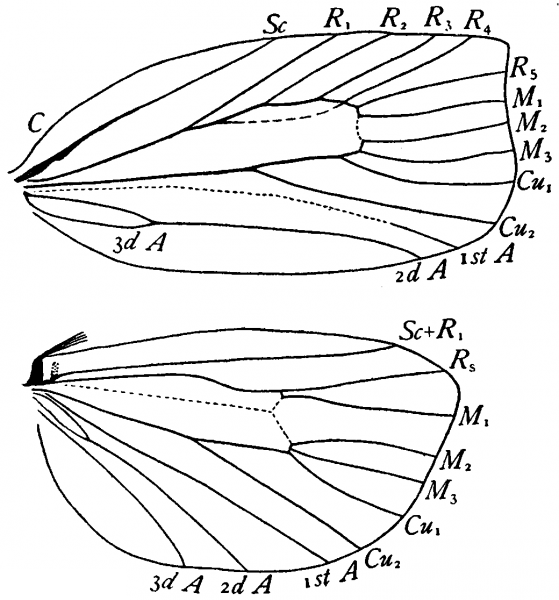
\includegraphics[width=\textwidth]{TortricidWings}
        \caption{Wings \citep[Fig. 353]{comstock1918wings}}
        \label{fig:tortricid1}
    \end{subfigure}
    \qquad %add desired spacing between images, e. g. ~, \quad, \qquad, \hfill etc. 
      %(or a blank line to force the subfigure onto a new line)
    \begin{subfigure}[ht!]{0.48\textwidth}
        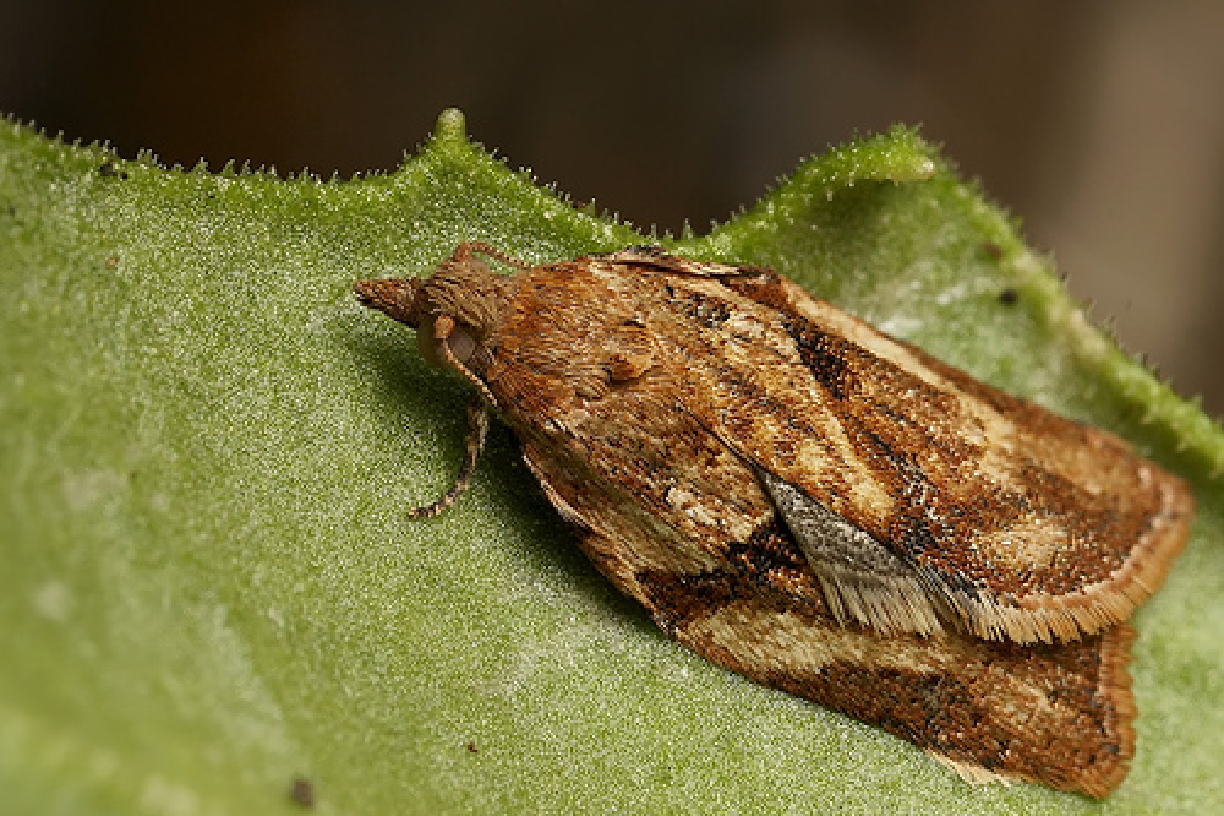
\includegraphics[width=\textwidth]{image45}
        \caption{Habitus}
        \label{fig:tortricid2}
    \end{subfigure}
    \caption{Tortricidae}\label{fig:tortricids}
\end{figure}

\subsubsection{Limacodidae (slug caterpillar moths)}
\begin{itemize}
\item stout-bodied
\item usually brown and green or brown and silver
\item fore wing with 2 complete anal veins
\item Sc and R in hind wing separate at base, then briefly fused 
\item hind wing with 3 anal veins
\end{itemize}

\begin{figure}[ht!]
    \centering
    \begin{subfigure}[ht!]{0.35\textwidth}
        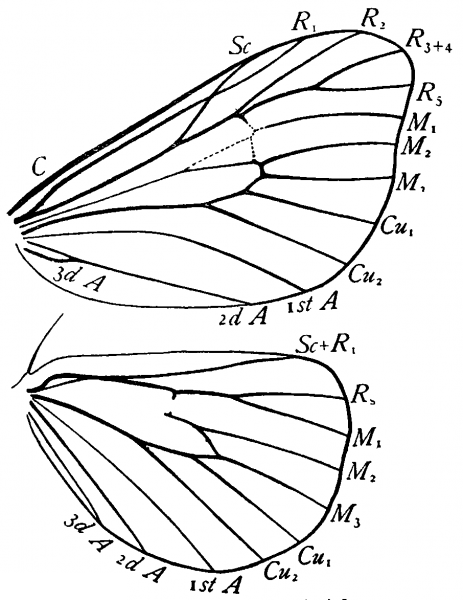
\includegraphics[width=\textwidth]{LimacodidWings}
        \caption{Wings \citep[Fig. 349]{comstock1918wings}}
        \label{fig:limacodid1}
    \end{subfigure}
    \qquad %add desired spacing between images, e. g. ~, \quad, \qquad, \hfill etc. 
      %(or a blank line to force the subfigure onto a new line)
    \begin{subfigure}[ht!]{0.48\textwidth}
        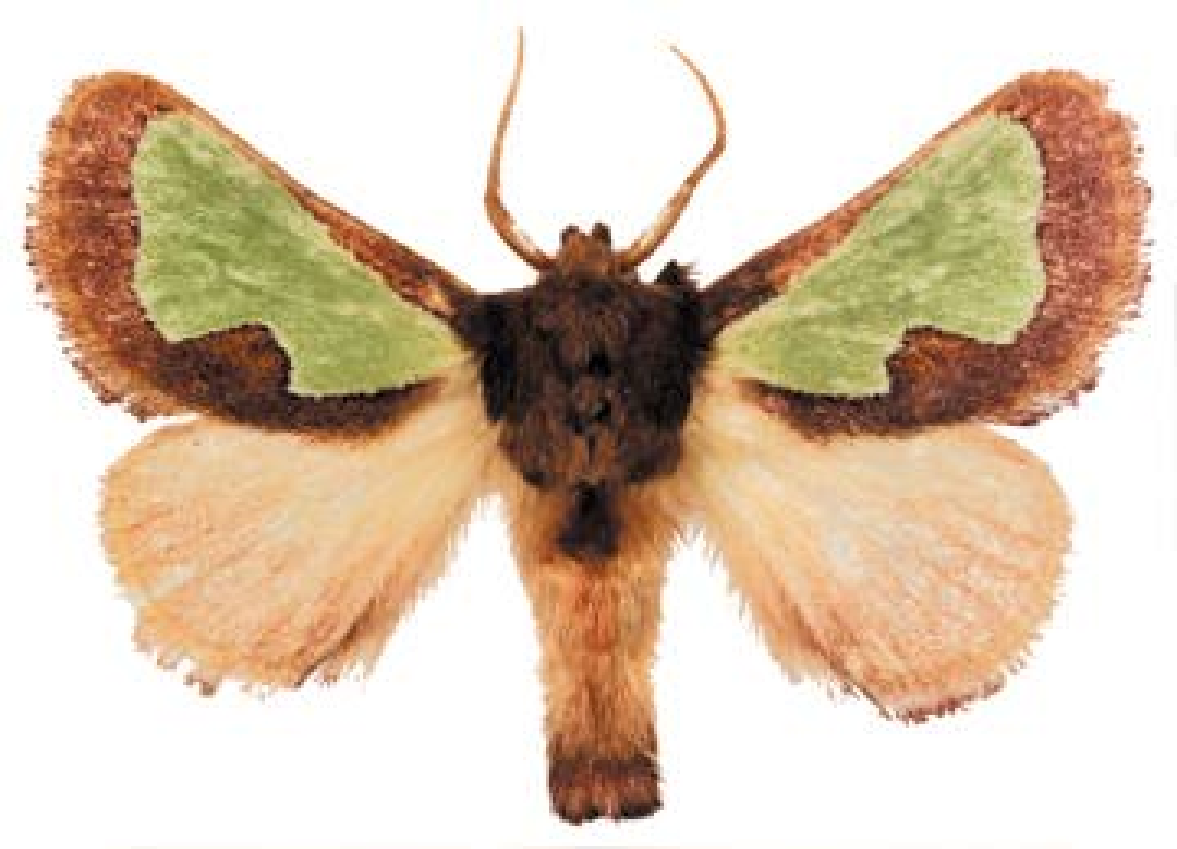
\includegraphics[width=\textwidth]{image47}
        \caption{Habitus}
        \label{fig:limacodid2}
    \end{subfigure}
    \caption{Limacodidae}\label{fig:limacodids}
\end{figure}

\subsubsection{Pyraloidea (snout moths and relatives)}
\begin{itemize}
\item fore wing usually elongate-triangular, hind wing more rounded and often broader
\item palps often large and projecting forward
\item proboscis scaly
\item tympana present on abdomen
\item Sc + R1 and Rs in hind wing fused beyond discal cell then separating (this character can be hard to see)
\item hind wing with 3 anal veins
\end{itemize}
% two families, difficult to separate in a lab like this, subtle characters

\begin{figure}[ht!]
    \centering
    \begin{subfigure}[ht!]{0.38\textwidth}
        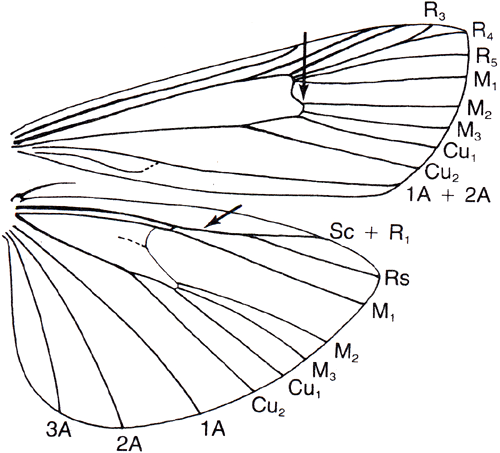
\includegraphics[width=\textwidth]{image20}
        \caption{Wings}
        \label{fig:pyraloid1}
    \end{subfigure}
    \qquad %add desired spacing between images, e. g. ~, \quad, \qquad, \hfill etc. 
      %(or a blank line to force the subfigure onto a new line)
    \begin{subfigure}[ht!]{0.48\textwidth}
        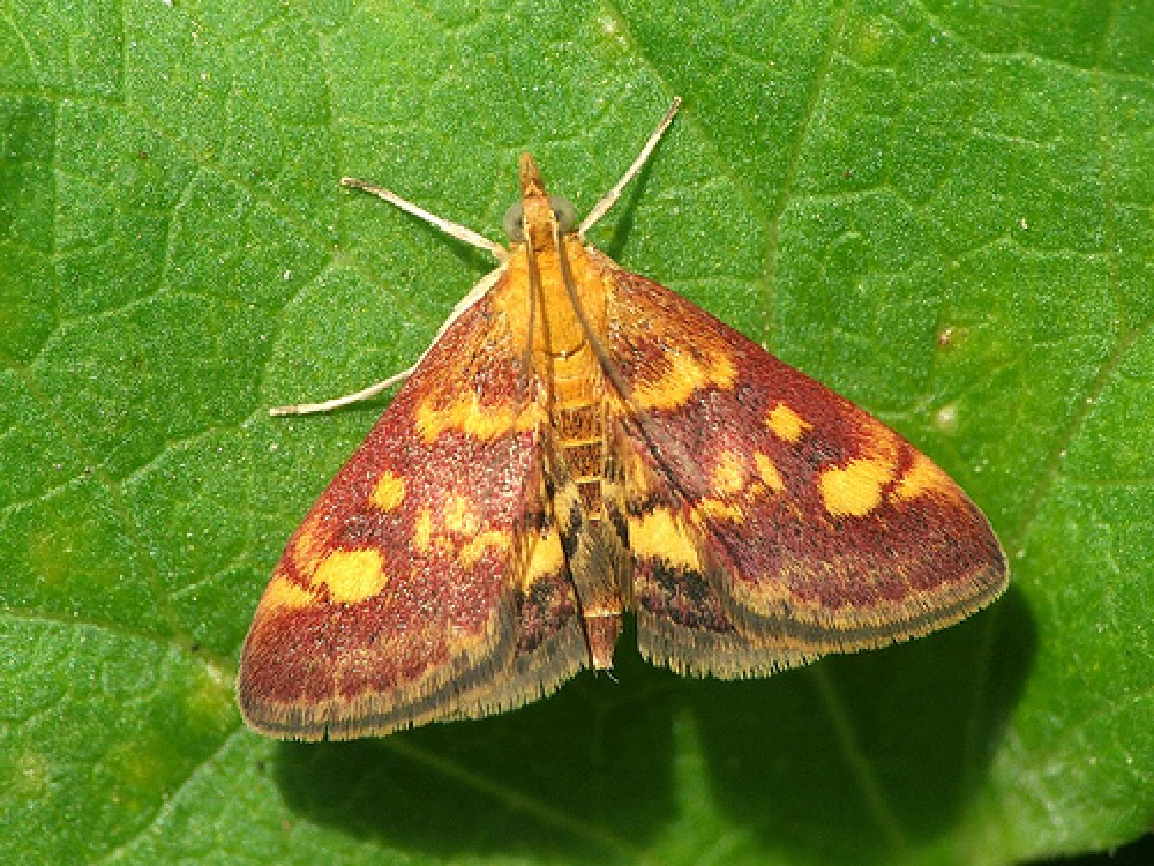
\includegraphics[width=\textwidth]{image19}
        \caption{Habitus}
        \label{fig:pyraloid2}
    \end{subfigure}
    \caption{Pyraloidea}\label{fig:pyraloids}
\end{figure}

\subsubsection{Geometridae (inchworms, spanworms, loopers, etc.)}
\begin{itemize}
\item somewhat butterfly-like in shape with broad wings, slender body but:
\item antennae threadlike or pectinate, not clubbed
\item proboscis bare
\item Sc in hind wing with an abrupt angle basally
\item usually cryptically colored
\item tympana at the base of the abdomen
\item the geometric patterns on the fore wings often continue onto the hind wing
\end{itemize}

\begin{figure}[ht!]
    \centering
    \begin{subfigure}[ht!]{0.35\textwidth}
        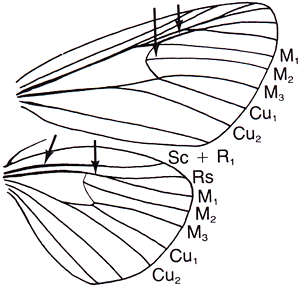
\includegraphics[width=\textwidth]{image17}
        \caption{Wings}
        \label{fig:geometrid1}
    \end{subfigure}
    \qquad %add desired spacing between images, e. g. ~, \quad, \qquad, \hfill etc. 
      %(or a blank line to force the subfigure onto a new line)
    \begin{subfigure}[ht!]{0.48\textwidth}
        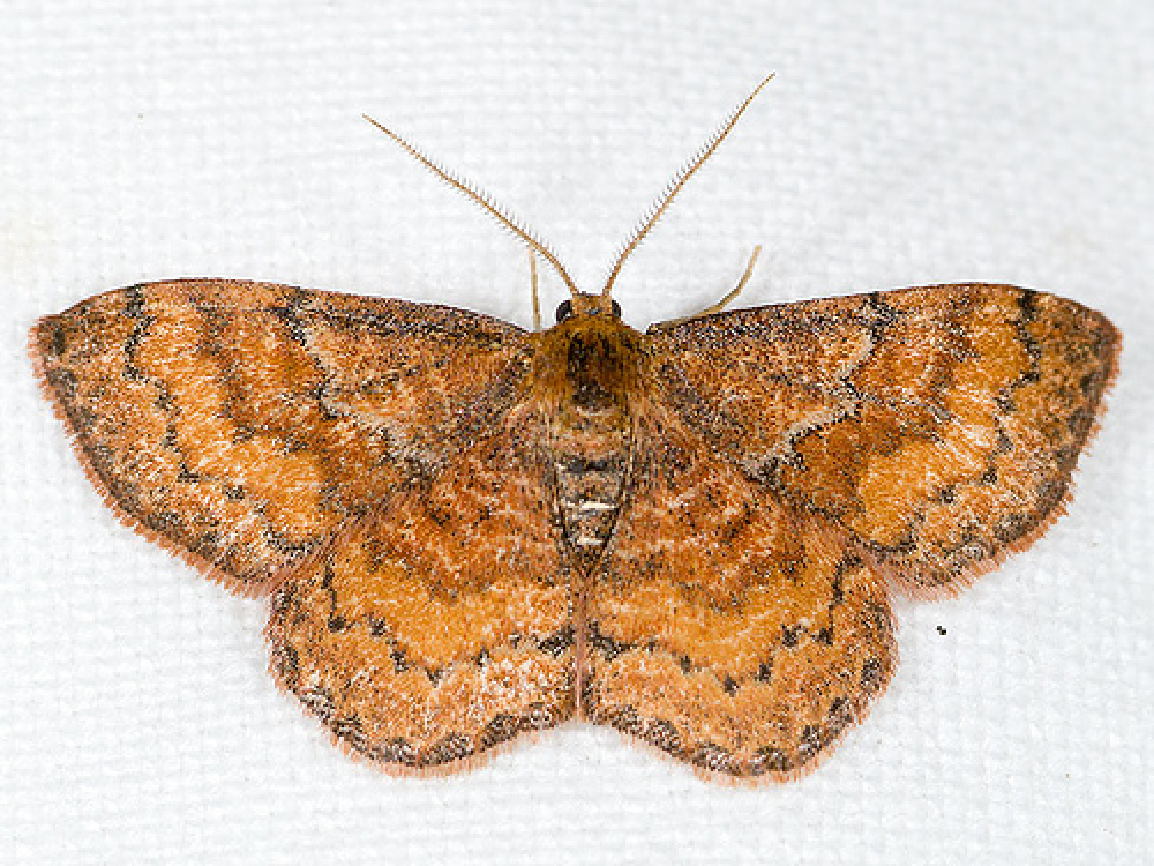
\includegraphics[width=\textwidth]{image22}
        \caption{Habitus}
        \label{fig:geometrid2}
    \end{subfigure}
    \caption{Geometridae}\label{fig:geometrids}
\end{figure}

\paragraph{Rhopalocera (butterflies)} The next five families are all commonly referred to as butterflies (although Hesperiidae is sometimes excluded). They can be recognized by the following characters:
\begin{itemize}
\item antennae knobbed/hooked at tip
\item ocelli always absent
\item body usually small relative to wings, wings usually broad
\item hind wing with only 1 or 2 anal veins
\end{itemize}

\subsubsection{Hesperiidae (skippers)}
\begin{itemize}
\item antennae clubbed but also hooked at tip 
\item antennal insertions widely separated
\item R in fore wing 5-branched
\item fairly stout-bodied compared to butterflies, with large, broad heads
\end{itemize}

\begin{figure}[ht!]
    \centering
    \begin{subfigure}[ht!]{0.31\textwidth}
        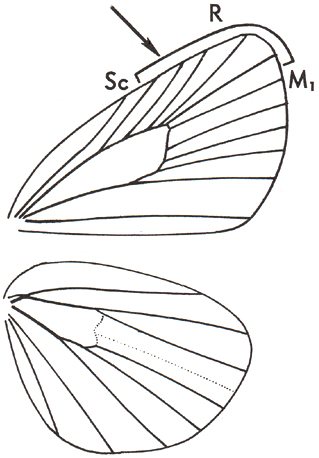
\includegraphics[width=\textwidth]{image25}
        \caption{Wings}
        \label{fig:hesperiid1}
    \end{subfigure}
    \qquad %add desired spacing between images, e. g. ~, \quad, \qquad, \hfill etc. 
      %(or a blank line to force the subfigure onto a new line)
    \begin{subfigure}[ht!]{0.5\textwidth}
        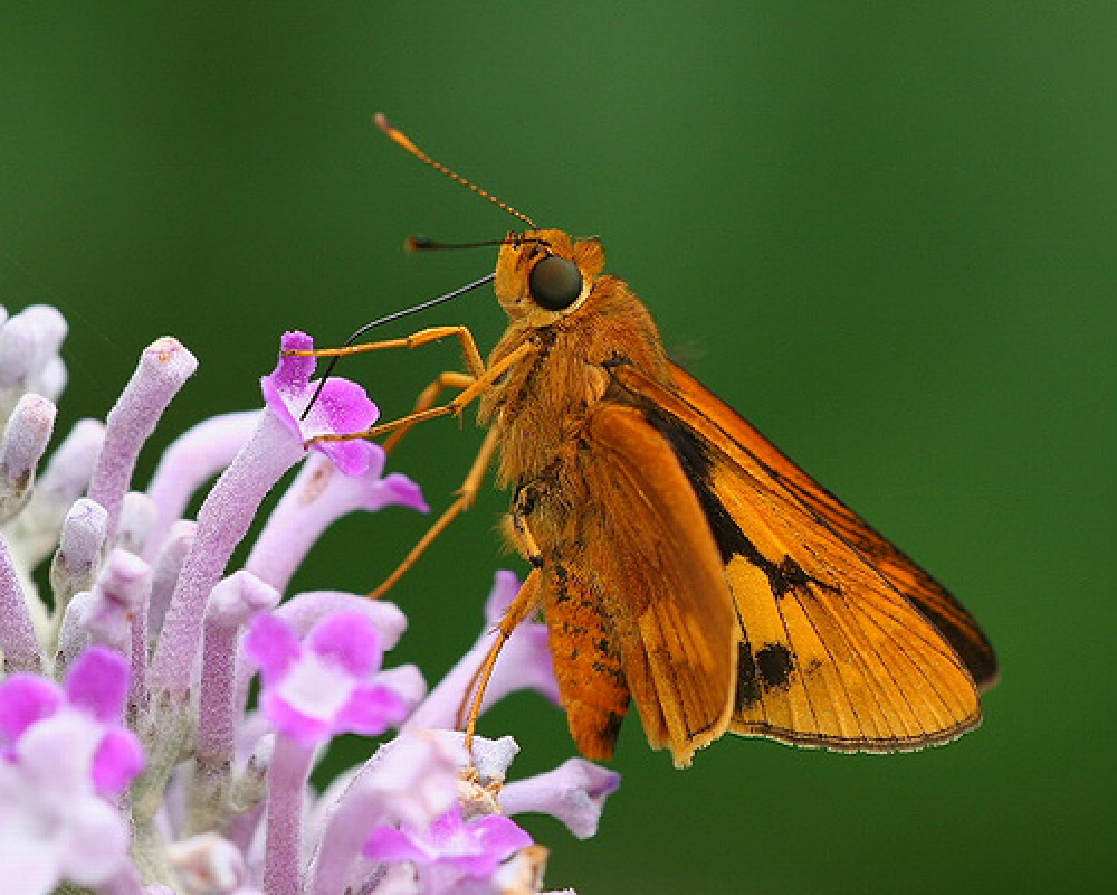
\includegraphics[width=\textwidth]{image24}
        \caption{Habitus}
        \label{fig:hesperiid2}
    \end{subfigure}
    \caption{Hesperiidae}\label{fig:hesperiids}
\end{figure}

\subsubsection{Papilionidae (swallowtails)}
\begin{itemize}
\item fore wing with R 5-branched
\item hind wing with 1 anal vein and usually with tail-like projection
\item 4 branches off Cu at bottom of discal cell
\item fore legs not reduced
\item usually brightly colored (black, yellow and other colors) and large
\end{itemize}

\begin{figure}[ht!]
    \centering
    \begin{subfigure}[ht!]{0.28\textwidth}
        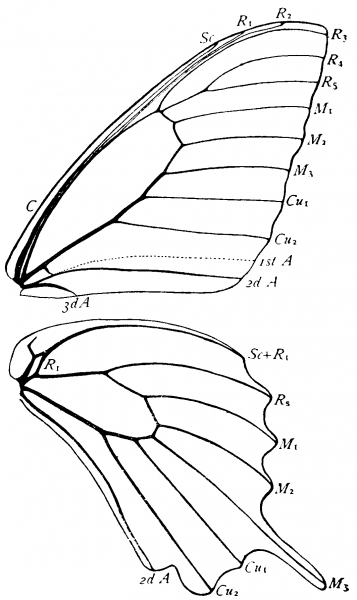
\includegraphics[width=\textwidth]{PapilionidWings}
        \caption{Wings \citep[Fig. 350]{comstock1918wings}}
        \label{fig:papilionid1}
    \end{subfigure}
    \qquad %add desired spacing between images, e. g. ~, \quad, \qquad, \hfill etc. 
      %(or a blank line to force the subfigure onto a new line)
    \begin{subfigure}[ht!]{0.5\textwidth}
        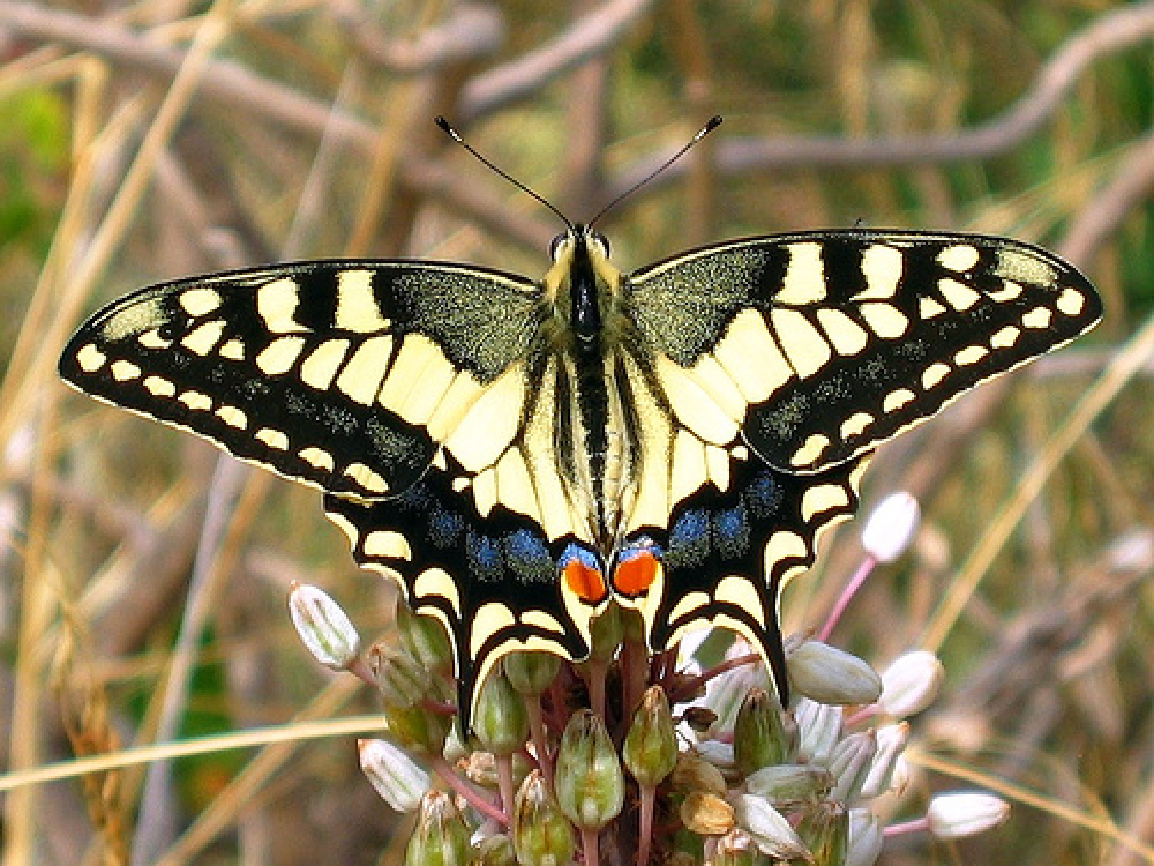
\includegraphics[width=\textwidth]{image27}
        \caption{Habitus}
        \label{fig:papilionid2}
    \end{subfigure}
    \caption{Papilionidae}\label{fig:papilionids}
\end{figure}

\subsubsection{Nymphalidae (brush-footed butterflies)}
\begin{itemize}
\item R 5-branched in fore wing
\item fore legs greatly reduced, lacking tarsal claws (rarely normal sized)
\item discal cell in hind wing often open or weakly closed
\item large or medium-sized, variable in color and shape
\end{itemize}

\begin{figure}[ht!]
    \centering
    \begin{subfigure}[ht!]{0.28\textwidth}
        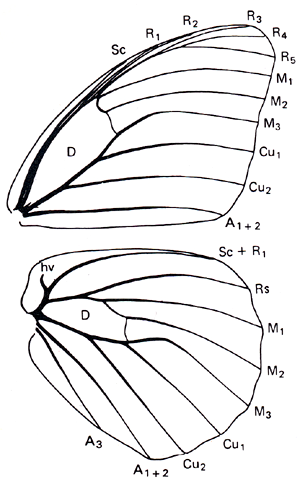
\includegraphics[width=\textwidth]{image09}
        \caption{Wings}
        \label{fig:nymphalid1}
    \end{subfigure}
    \qquad %add desired spacing between images, e. g. ~, \quad, \qquad, \hfill etc. 
      %(or a blank line to force the subfigure onto a new line)
    \begin{subfigure}[ht!]{0.5\textwidth}
        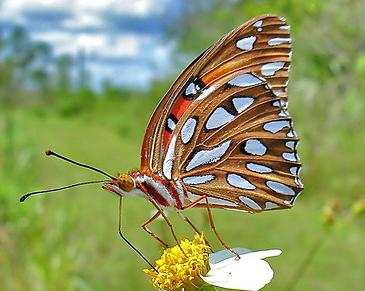
\includegraphics[width=\textwidth]{image28}
        \caption{Habitus}
        \label{fig:nymphalid2}
    \end{subfigure}
    \caption{Nymphalidae}\label{fig:nymphalids}
\end{figure}

\subsubsection{Pieridae (whites and sulfurs)}
\begin{itemize}
\item R 3–5-branched in fore wing
\item hind wing with 2 anal veins and no tail
\item front legs not or only slightly reduced
\item M1 of fore wing stalked with a branch of R near wing tip
\item medium sized and usually white, yellow or orange marked with black or plain
\end{itemize}

\begin{figure}[ht!]
    \centering
    \begin{subfigure}[ht!]{0.25\textwidth}
        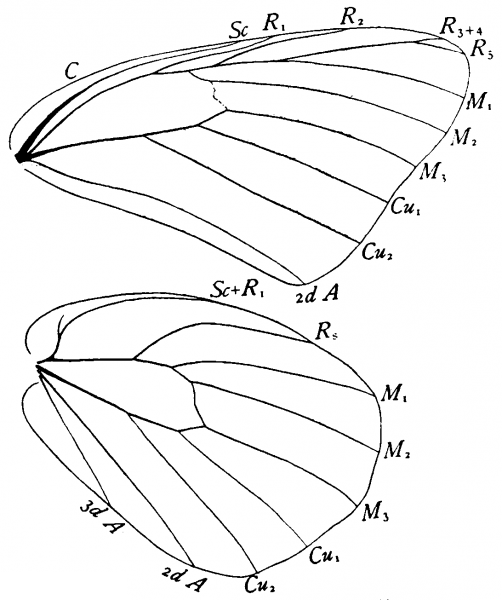
\includegraphics[width=\textwidth]{PieridWings}
        \caption{Wings \citep[Fig. 342]{comstock1918wings}}
        \label{fig:pierid1}
    \end{subfigure}
    \qquad %add desired spacing between images, e. g. ~, \quad, \qquad, \hfill etc. 
      %(or a blank line to force the subfigure onto a new line)
    \begin{subfigure}[ht!]{0.5\textwidth}
        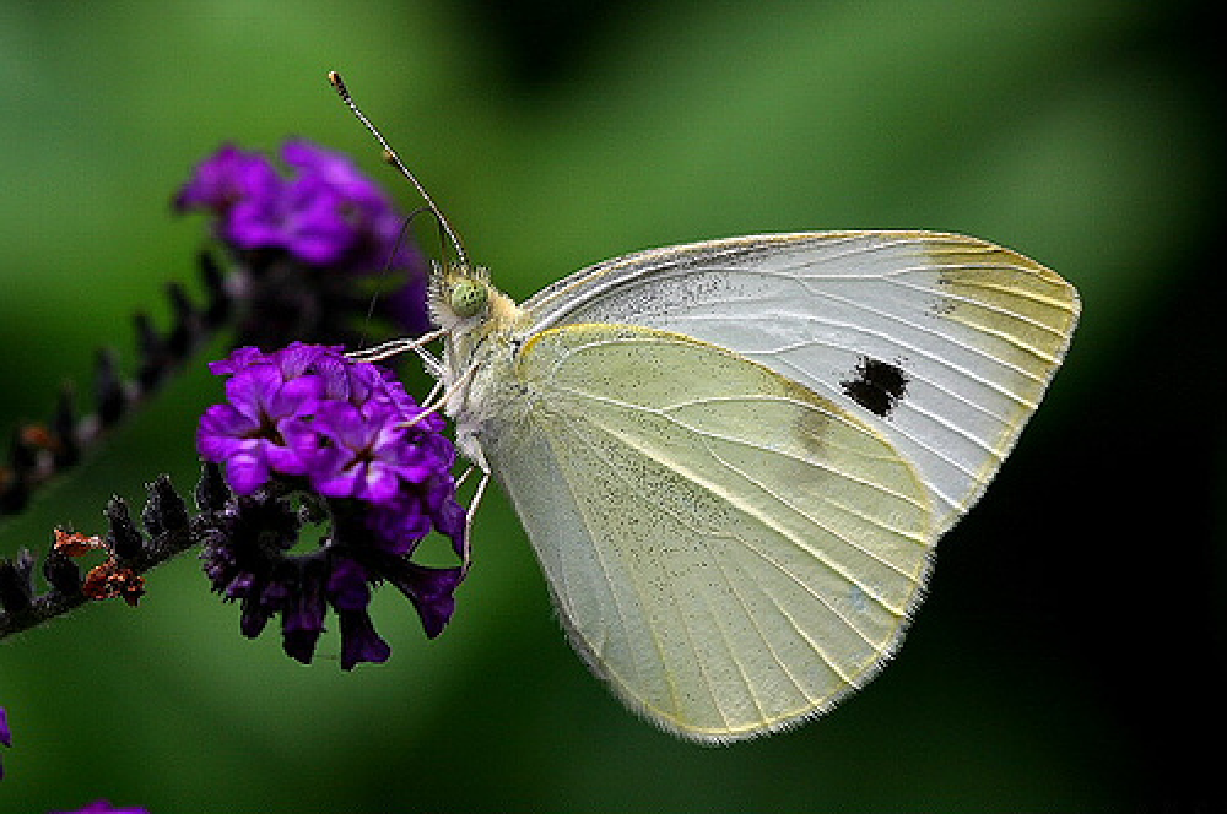
\includegraphics[width=\textwidth]{image11}
        \caption{Habitus}
        \label{fig:pierid2}
    \end{subfigure}
    \caption{Pieridae}\label{fig:pierids}
\end{figure}

\subsubsection{Lycaenidae (blues, coppers, hairstreaks)}
\begin{itemize}
\item R 3-4-branched in fore wing
\item hind wing with 2 anal veins, occasionally with very tiny hair-like tail
\item M1 of fore wing very rarely stalked with a branch of R near wing tip
\item front legs of males sometimes strongly reduced
\item small, very delicate and often brightly colored but usually not white or yellow, antennae often striped
\end{itemize}

\begin{figure}[ht!]
    \centering
    \begin{subfigure}[ht!]{0.28\textwidth}
        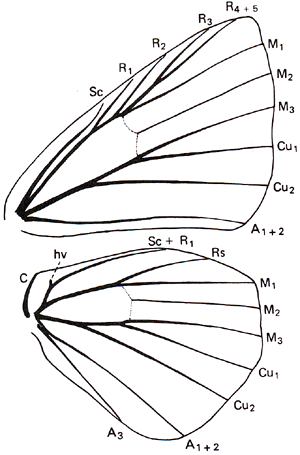
\includegraphics[width=\textwidth]{image13}
        \caption{Wings}
        \label{fig:lycaenid1}
    \end{subfigure}
    \qquad %add desired spacing between images, e. g. ~, \quad, \qquad, \hfill etc. 
      %(or a blank line to force the subfigure onto a new line)
    \begin{subfigure}[ht!]{0.4\textwidth}
        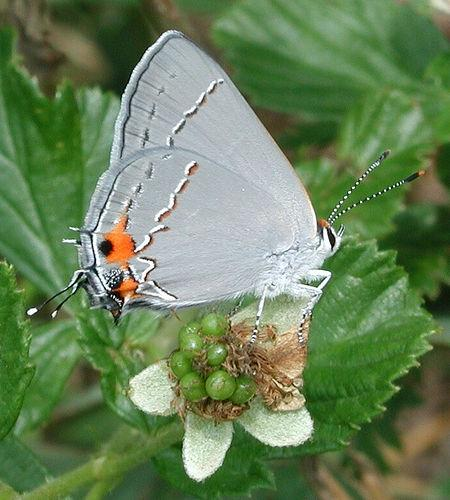
\includegraphics[width=\textwidth]{image12}
        \caption{Habitus}
        \label{fig:lycaenid2}
    \end{subfigure}
    \caption{Lycaenidae}\label{fig:lycaenids}
\end{figure}

\paragraph{Macrolepidoptera (excluding Rhopalocera)} The remaining families are moths that tend to be relatively large and generally share these characters: 
\begin{itemize}
\item hind wing with only 1 or 2 anal veins
\item fore wing with 1 anal vein reaching margin
\end{itemize}

\subsubsection{Sphingidae (hawk moths)}
\begin{itemize}
\item antennae thickened, somewhat spindle-shaped
\item fore wings narrow, usually much larger than hind wings
\item small crossvein at midlength along top of discal cell in hind wing
\item proboscis long, prominent
\item no ocelli or tympanal organs
\item often large, body very robust, abdomen often pointed
\end{itemize}

\begin{figure}[ht!]
    \centering
    \begin{subfigure}[ht!]{0.35\textwidth}
        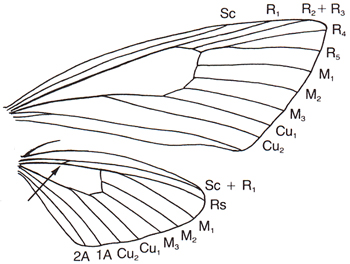
\includegraphics[width=\textwidth]{image15}
        \caption{Wings}
        \label{fig:sphingid1}
    \end{subfigure}
    \qquad %add desired spacing between images, e. g. ~, \quad, \qquad, \hfill etc. 
      %(or a blank line to force the subfigure onto a new line)
    \begin{subfigure}[ht!]{0.4\textwidth}
        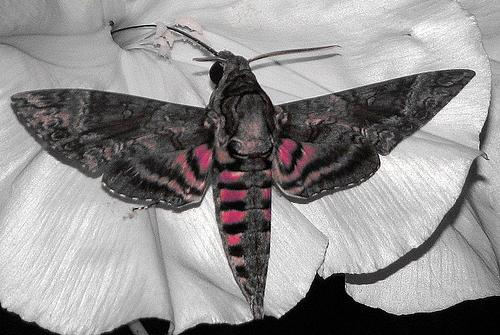
\includegraphics[width=\textwidth]{image14}
        \caption{Habitus}
        \label{fig:sphingid2}
    \end{subfigure}
    \caption{Sphingidae}\label{fig:sphingids}
\end{figure}

\subsubsection{Saturniidae (giant silk moths)}
\noindent{}\textit{Diagnostic characters:} Antennae often bipectinate; no basal areole in hind wing; fore wing M2 arising closer to M1 than M3; hind wing Sc and Rs not fused; frenulum absent; proboscis reduced or absent; medium-sized to large (wingspan up to 15 cm), with broad wings and short, thick bodies.\\

\noindent{}\textit{Natural history:} 

\begin{figure}[ht!]
    \centering
    \begin{subfigure}[ht!]{0.31\textwidth}
        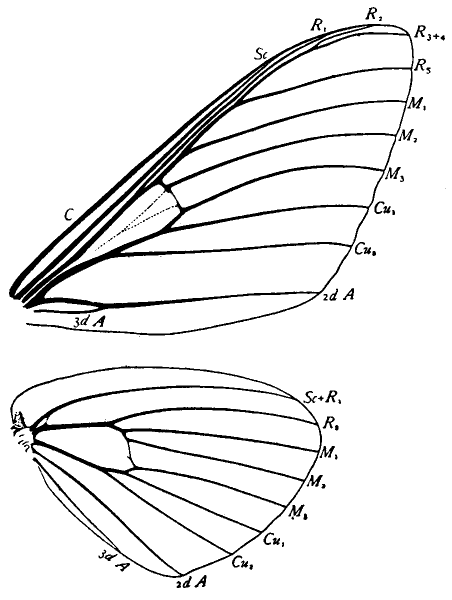
\includegraphics[width=\textwidth]{SaturniidWings}%fig 345 from comstock 1918
        \caption{Wings \citep[Fig. 345]{comstock1918wings}}
        \label{fig:saturniid1}
    \end{subfigure}
    ~ %add desired spacing between images, e. g. ~, \quad, \qquad, \hfill etc. 
      %(or a blank line to force the subfigure onto a new line)
    \begin{subfigure}[ht!]{0.48\textwidth}
        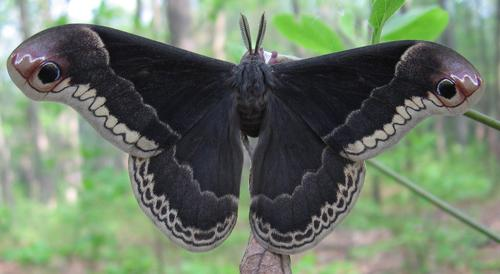
\includegraphics[width=\textwidth]{image00}
        \caption{Habitus}
        \label{fig:saturniid2}
    \end{subfigure}
    \caption{Saturniidae}\label{fig:saturniids}
\end{figure}

\subsubsection{Lasiocampidae (tent caterpillars, lappet moths, eggars)}
\noindent{}\textit{Diagnostic characters:} Antennae bipectinate; proboscis vestigial or absent; fore wing Cu2 arising near wing base; basal areole present in hind wing; frenulum absent, humeral area of hind wing greatly expanded; fore wing M2 arising closer to M3 than M1; relatively fat-bodied and hairy moths.\\

\noindent{}\textit{Natural history:} Caterpillars diversely phytophagous but mostly on leaves of trees and shrubs. caterpillars setose, often with flattened evaginations (flaps or ``lappets'') near prolegs. Some species live communally in tents during the larval stages.

\begin{figure}[ht!]
    \centering
    \begin{subfigure}[ht!]{0.3\textwidth}
        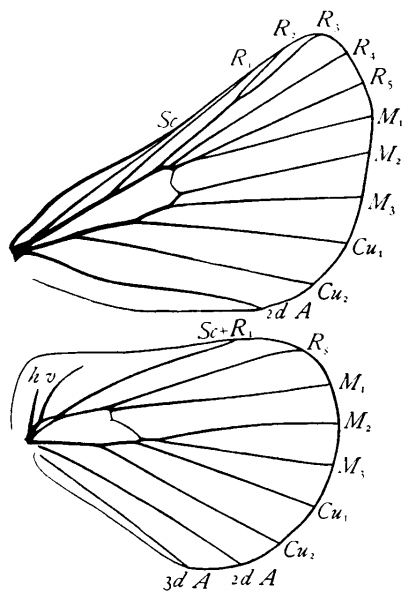
\includegraphics[width=\textwidth]{LasiocampidWings}
        \caption{Wings \citep[Fig. 69]{comstock1918wings}}
        \label{fig:lasiocampid1}
    \end{subfigure}
    \qquad %add desired spacing between images, e. g. ~, \quad, \qquad, \hfill etc. 
      %(or a blank line to force the subfigure onto a new line)
    \begin{subfigure}[ht!]{0.31\textwidth}
        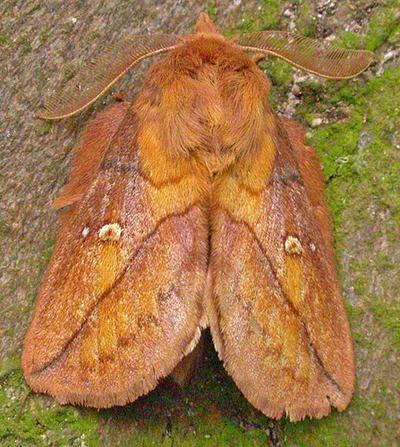
\includegraphics[width=\textwidth]{image01}
        \caption{Habitus}
        \label{fig:lasiocampid2}
    \end{subfigure}
    \caption{Lasiocampidae}\label{fig:lasiocampids}
\end{figure}

\subsubsection{Notodontidae (prominents)}
\noindent{}\textit{Diagnostic characters:} Antennae usually bipectinate, occasionally simple; tympanum on metathorax pointing ventrally; tympanal hood absent; no basal areole in hind wing; Sc and Rs in hind wing parallel, not fused; fore wing M2 arising in midway between M1 and M3 (key character to separate from Noctuidae and Erebidae); fore wing usually conspicuously longer than hind wing; body relatively stout, usually drab-colored.\\

\noindent{}\textit{Natural history:} There are almost 4,000 species of prominents worldwide. Larvae typically feed on trees and have a distinctive habitus. Adults do not feed.

\begin{figure}[ht!]
    \centering
    \begin{subfigure}[ht!]{0.32\textwidth}
        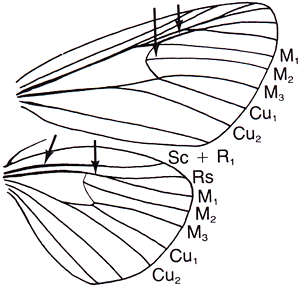
\includegraphics[width=\textwidth]{image17}
        \caption{Wings}
        \label{fig:notodontid1}
    \end{subfigure}
    \qquad %add desired spacing between images, e. g. ~, \quad, \qquad, \hfill etc. 
      %(or a blank line to force the subfigure onto a new line)
    \begin{subfigure}[ht!]{0.44\textwidth}
        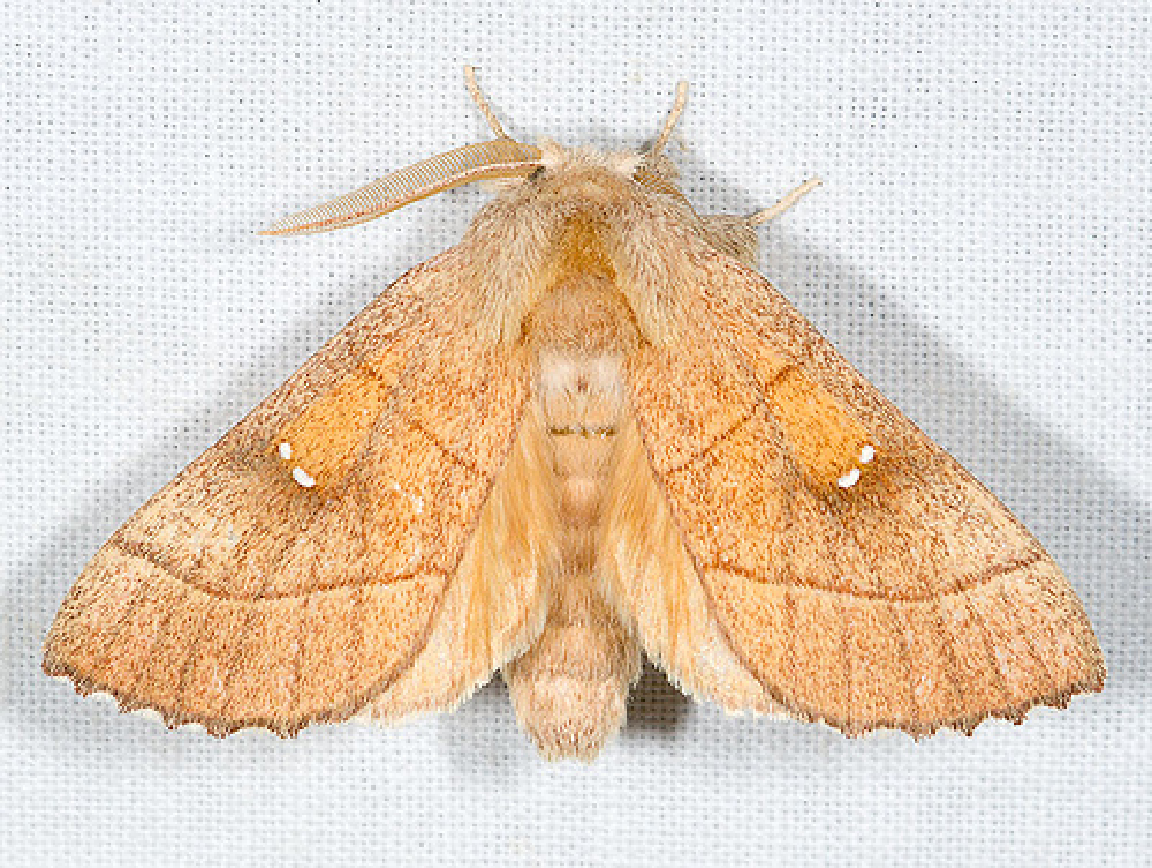
\includegraphics[width=\textwidth]{image16}
        \caption{Habitus}
        \label{fig:notodontid2}
    \end{subfigure}
    \caption{Notodontidae}\label{fig:notodontids}
\end{figure}

\subsubsection{Noctuidae (owlet moths)}
\noindent{}\textit{Diagnostic characters:} Antennae usually simple, occasionally bipectinate, sometimes swollen apically; tympanum on metathorax pointing posteriorly or outwards; tympanal hood located posterior to spiracle; labial palps usually relatively long, upturned; ocelli sometimes present, medium-sized to large; fore wings usually cryptic, sometimes with eye-like  spots; hind wing cubital vein branches into 2 or 3 veins (\textbf{hind wing trifine or bifine}); body color usually dominated by browns.\\

\noindent{}\textit{Natural history:} Hugely diverse taxon, with tens of thousands of species; its taxonomic limits remain unsettled. Their natural history is difficult to generalize, but these moths are typically night-fliers. Larvae are diversely herbivorous and include many important pest species.

\begin{figure}[ht!]
    \centering
    \begin{subfigure}[ht!]{0.37\textwidth}
        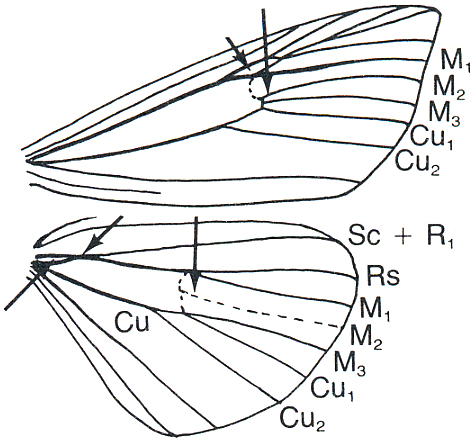
\includegraphics[width=\textwidth]{image08}
        \caption{Wings}
        \label{fig:noctuid1}
    \end{subfigure}
    \qquad %add desired spacing between images, e. g. ~, \quad, \qquad, \hfill etc. 
      %(or a blank line to force the subfigure onto a new line)
    \begin{subfigure}[ht!]{0.37\textwidth}
        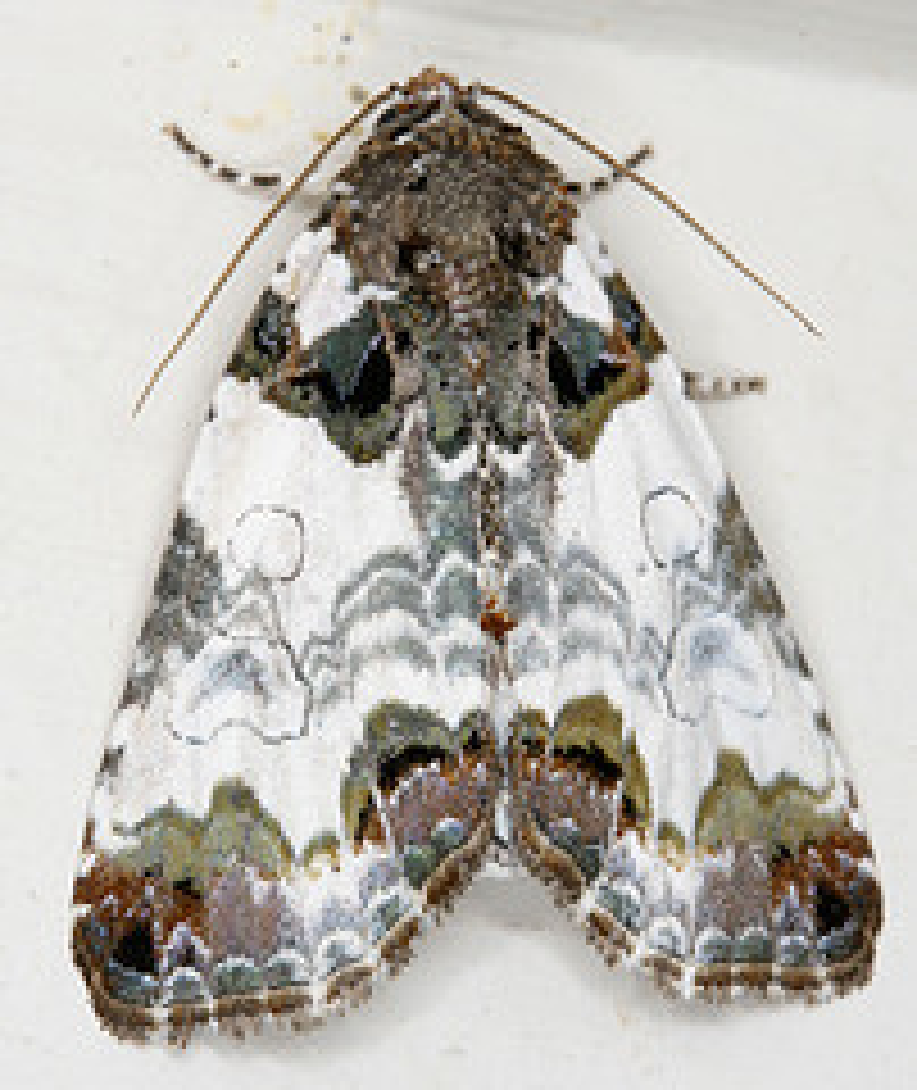
\includegraphics[width=\textwidth]{image07}
        \caption{Habitus}
        \label{fig:noctuid2}
    \end{subfigure}
    \caption{Noctuidae}\label{fig:noctuids}
\end{figure}

\subsubsection{Erebidae (includes Lymantriidae, Arctiidae, and several lineages that used to be in Noctuidae)}
\noindent{}\textit{Diagnostic characters:} Similar to Noctuidae but hind wing cubital vein branches into 4 veins: CU2, CU1, M3, M2 (\textit{i.e.}, \textbf{hind wing quadrifine})\\

\noindent{}\textit{Natural history:} Like Noctuidae, this is a hugely diverse taxon, with tens of thousands of species. Their natural history is difficult to generalize, but these moths are typically night-fliers. Larvae are diversely herbivorous and include many important pest species.

\begin{figure}[ht!]
    \centering
    \begin{subfigure}[ht!]{0.38\textwidth}
        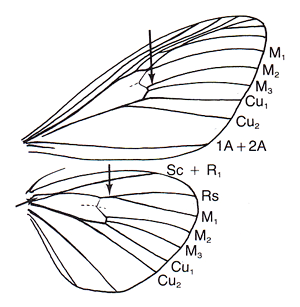
\includegraphics[width=\textwidth]{image04}
        \caption{Wings}
        \label{fig:erebid1}
    \end{subfigure}
    \qquad %add desired spacing between images, e. g. ~, \quad, \qquad, \hfill etc. 
      %(or a blank line to force the subfigure onto a new line)
    \begin{subfigure}[ht!]{0.38\textwidth}
        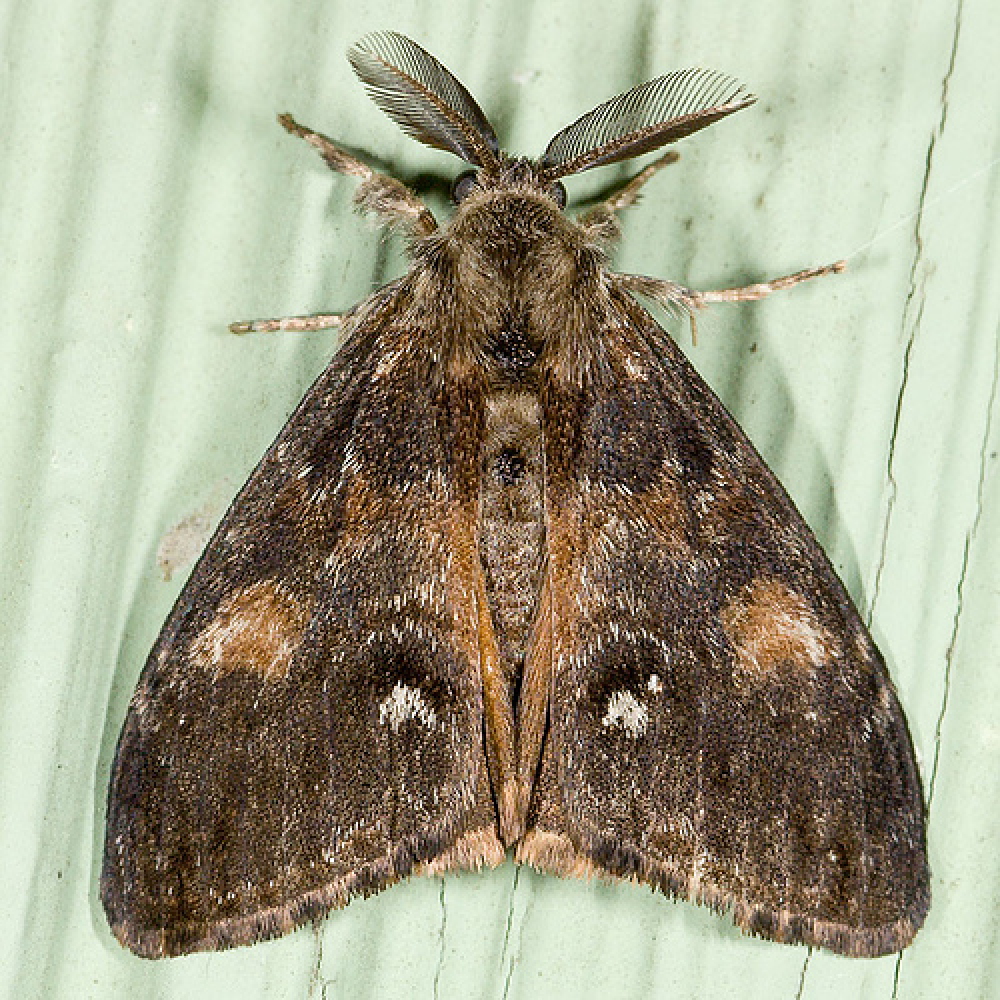
\includegraphics[width=\textwidth]{image03}
        \caption{Habitus}
        \label{fig:erebid2}
    \end{subfigure}
    \caption{Erebidae}\label{fig:erebids}
\end{figure}

\FloatBarrier
\section{Trichoptera}

\noindent{}\textbf{Trichoptera} comprises approximately 13,000 species,  %http://www.mapress.com/zootaxa/2007f/zt01668p698.pdf
the vast majority of which are aquatic as larvae. Larvae exhibit diverse life history strategies and serve as important indicators of environmental health. For these reasons, we'll be examining larval specimens alongside adults. Larvae use silk extensively, often constructing static or portable shelters. Adult mouthparts are diagnostic for the order, being heighly reduced (haustellum) but with long palpi.

\subsection*{Big picture questions}

\noindent{}This is the most diverse aquatic taxon. What factors contribute to their overall diversity, compared to Odonata, Ephemeroptera, and Plecoptera?\\

\noindent{}Can you describe one or two characteristics that could be key innovations or opportunities?\\

\noindent{}With mouthpart modification another non-feeding related but vital function was lost. Can you describe an evolutionary novelty gained by trichopterans during the course of evolution that solves some problems associated with mandible reduction?\\

\noindent{}What trends do we see across the phylogeny of Trichoptera, with respect to feeding biology and silk use? \\

\noindent{}Familiarize yourself with the following taxon names, which refer to organisms you are likely to encounter in the northeastern USA and/or which are phylogenetically relevant. Can you describe how these arthropods live (natural history) and roughly how diverse they are? Do you know how they're related to one another? If you had to choose a taxon to study which one would it be and why?
\begin{enumerate} 
\item Annulipalpia
\item Hydropsychidae
\item Hydroptilidae
\item Integripalpia
\end{enumerate}

\begin{figure}[ht!]
  \centering
    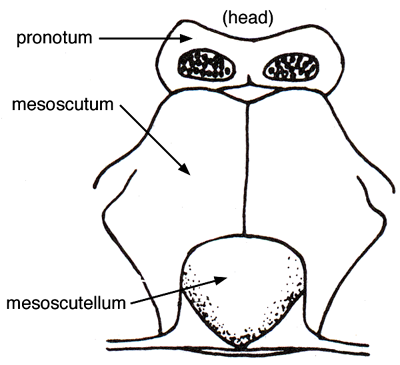
\includegraphics[width=0.4\textwidth]{TrichoImage03}
  \caption{Trichoptera, pro- and mesothorax, in dorsal view}
  \label{fig:caddisthorax}
\end{figure}

\subsection{Hydroptilidae (micro-caddisflies)}
\noindent{}\textit{Diagnostic characters:} antennae short, mesoscutum without warts, fore tibiae with 1 spur, very small (usually less than 5 mm), usually mottled grayish or brownish and very hairy.\\

\noindent{}\textit{Natural history:} These insects are among the smallest trichopterans, rarely measuring \textgreater5 mm as adults. Larvae are free-living until the final instar, which builds a silken structure referred to as a ``purse case''. Larvae feed on filamentous algae and/or diatoms.

\begin{figure}[ht!]
  \centering
    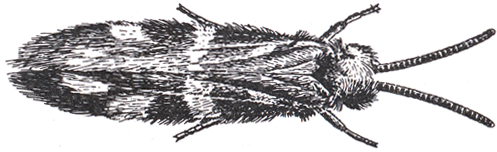
\includegraphics[width=0.6\textwidth]{TrichoImage05}
  \caption{Hydoptilidae}
  \label{fig:hydrop}
\end{figure}

\subsection{Hydropsychidae (net-spinning caddisflies)}
\noindent{}\textit{Diagnostic characters:} antennae long but usually less than 2$\times$ body; ocelli absent; maxillary palp 5-segmented, with apical segment longer than preceding segments; mesoscutum without warts; fore tibiae without preapical spurs.\\

\noindent{}\textit{Natural history:} Larvae construct trumpet-shaped retreats, attached to rocks in lotic environments. Detritus and invertebrates that get caught in these nets serve as forage for these caddisfly larvae. 

\begin{figure}[ht!]
  \centering
    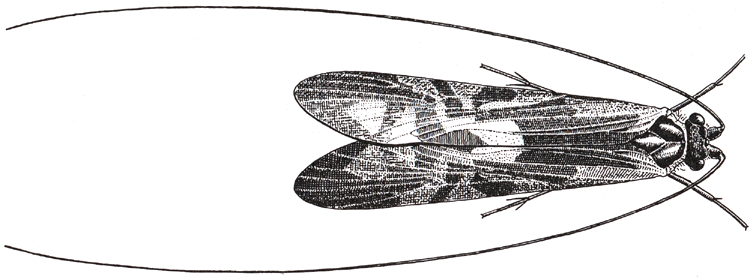
\includegraphics[width=0.6\textwidth]{TrichoImage04}
  \caption{Hydropsychidae}
  \label{fig:hydropsy}
\end{figure}

\subsection{Leptoceridae (long-horned caddisflies)}%http://bmcevolbiol.biomedcentral.com/articles/10.1186/1471-2148-11-10
\noindent{}\textit{Diagnostic characters:} body slender, small to medium-sized; \textbf{antennae hair-like, usually 2$\times$ body length}; ocelli absent; pronotum with a pair (or 2) of warts separated by notch; dorsal mesoscutum with 2 bands of setiferous punctures instead of setal warts.\\

\noindent{}\textit{Natural history:} Larvae mostly detritivorous shredders and algae (periphyton) scrapers; some species predators. Larvae, which also have relatively long antennae, typically construct tubular cases.

\begin{figure}[ht!]
    \centering
    \begin{subfigure}[ht!]{0.6\textwidth}
        \includegraphics[width=\textwidth]{TrichoImage06}
        \caption{Habitus}
        \label{fig:lepto1}
    \end{subfigure}
    ~ %add desired spacing between images, e. g. ~, \quad, \qquad, \hfill etc. 
      %(or a blank line to force the subfigure onto a new line)
    \begin{subfigure}[ht!]{0.2\textwidth}
        \includegraphics[width=\textwidth]{TrichoImage07}
        \caption{Pro- and mesothorax}
        \label{fig:lepto2}
    \end{subfigure}
    \caption{Leptoceridae}\label{fig:leptoc}
\end{figure}

\subsection{Phryganeidae (large caddisflies)}
\noindent{}\textit{Diagnostic characters:} Antennae usually about as long as body; ocelli present; fore tibiae with 2 or more spurs; middle tibiae with 4 spurs; male maxillary palp 4-segmented; among the largest caddisflies; often mottled and brown.\\

\noindent{}\textit{Natural history:} Larvae make portable cases from a diverse array of materials and can usually be found in cold, lentic environments. Larvae are mostly detritivores.

\begin{figure}[ht!]
    \centering
    \begin{subfigure}[ht!]{0.6\textwidth}
        \includegraphics[width=\textwidth]{TrichoImage00}
        \caption{Habitus}
        \label{fig:phrygan1}
    \end{subfigure}
    ~ %add desired spacing between images, e. g. ~, \quad, \qquad, \hfill etc. 
      %(or a blank line to force the subfigure onto a new line)
    \begin{subfigure}[ht!]{0.25\textwidth}
        \includegraphics[width=\textwidth]{TrichoImage01}
        \caption{Palp}
        \label{fig:phrygan2}
    \end{subfigure}
    \caption{Phryganeidae}\label{fig:phrygan}
\end{figure}

\subsection{Limnephilidae (northern caddisflies)}
%\begin{multicols}{2}
\noindent{}\textit{Diagnostic characters:} Antennae usually about as long as body; ocelli present; fore tibiae with 1 spur or none; middle tibiae with 2 or 3 spurs; male maxillary palp 3-segmented, also often large; body usually brown with dark markings.\\ 

\noindent{}\textit{Natural history:} Larvae make portable cases from a diverse array of materials, and they graze on algae or scavenge. This family also includes some unusual species that are terrestrial. \\

%\end{multicols}

\begin{figure}[ht!]
  \centering
    \includegraphics[width=0.7\textwidth]{TrichoImage02}
  \caption{Limnephilidae. Photo (CC BY-NC 2.0) by Lynette \url{https://flic.kr/p/aTNQJZ}}
  \label{fig:phryg}
\end{figure}

% adding bibliography here
\bibliographystyle{apalike}
\bibliography{bib}

\end{document}
